\chapter{Business Intelligence Workload}

\section{Choke Points}
\chapter{Choke Points}
\label{sec:choke-points}

\newcommand{\tpcCard}[1]{\colorbox{lightgray}{\tt TPC-H #1}}
\newcommand{\cpSection}[4][]{%
	\subsection*{%
		CP-#2: [#3] #4%
		\ifthenelse{\equal{#1}{}}{}{\hfill \tpcCard{#1}}%
	}%
	\label{choke_point_#2}}

%%%%%%%%%%%%%%%%%%%%%%%%%%%%%%%%%%%%%%%%%%%%%%%%%%%%%%%%%%%%%%%%%%%%%%%%%%%%%%
%%%%%%%%%%%%%%%%%%%%%%%%%%%%%%%%%%%%%%%%%%%%%%%%%%%%%%%%%%%%%%%%%%%%%%%%%%%%%%
%%%%%%%%%%%%%%%%%%%%%%%%%%%%%%%%%%%%%%%%%%%%%%%%%%%%%%%%%%%%%%%%%%%%%%%%%%%%%%

\section*{Introduction}

Choke points are a superset of~\cite{LdbcDeliverable} with the exception of CP \chokePoint{7.1}, which was removed and replaced with a new choke point. The correlations between choke points and queries are displayed in \autoref{tab:query_choke_point}.

{
\setlength{\tabcolsep}{.1em}
% Template-based generation of the table showing choke point coverage by queries.
% Note that 'update' queries (DEL, INS) and their choke points (CP-9.x) are omitted from the table
\begin{table}[htbp]
\scriptsize
\centering
\begin{tabular}{|l|
    
        |c|
    
} \hline

    
        & \chokePoint{ {{- choke_point -}} }
    
 \\ \hline


    {#- only list queries that have at least on choke point -#}
    
        \hline
        \queryRefCard{ {{- query.0 -}} }{
            IC
            BI
            
        }{ {{- query.3 -}} }
        
            
                &  \yes  
            
         \\ \hline
    


\end{tabular}
\caption{Coverage of choke points by queries.}
\label{tab:query_choke_point}
\end{table}

}

%%%%%%%%%%%%%%%%%%%%%%%%%%%%%%%%%%%%%%%%%%%%%%%%%%%%%%%%%%%%%%%%%%%%%%%%%%%%%%
%%%%%%%%%%%%%%%%%%%%%%%%%%%%%%%%%%%%%%%%%%%%%%%%%%%%%%%%%%%%%%%%%%%%%%%%%%%%%%
%%%%%%%%%%%%%%%%%%%%%%%%%%%%%%%%%%%%%%%%%%%%%%%%%%%%%%%%%%%%%%%%%%%%%%%%%%%%%%

\section{Aggregation Performance}

%%%%%%%%%%%%%%%%%%%%%%%%%%%%%%%%%%%%%%%%%%%%%%%%%%%%%%%%%%%%%%%%%%%%%%%%%%%%%%

\cpSection[1.2]{1.1}{QOPT}{Interesting orders}

This choke point tests the ability of the query optimizer to exploit the interesting orders induced by some operators. Apart from clustered indexes providing key order, other operators also preserve or even induce tuple orderings.
Sort-based operators create new orderings, typically the probe-side of a hash join conserves its order, etc.

\subsubsection{Queries}
{\raggedright
\queryRefCard{bi-read-02}{BI}{2}
\queryRefCard{bi-read-04}{BI}{4}
\queryRefCard{bi-read-11}{BI}{11}
\queryRefCard{bi-read-17}{BI}{17}
\queryRefCard{bi-read-18}{BI}{18}
\queryRefCard{bi-read-19}{BI}{19}
\queryRefCard{interactive-complex-read-02}{IC}{2}
\queryRefCard{interactive-complex-read-09}{IC}{9}

}

%%%%%%%%%%%%%%%%%%%%%%%%%%%%%%%%%%%%%%%%%%%%%%%%%%%%%%%%%%%%%%%%%%%%%%%%%%%%%%

\cpSection[1.1]{1.2}{QEXE}{High cardinality group-by performance}

This choke point tests the ability of the execution engine to parallelize group-by's with a large number of groups. Some queries require performing large group-by's.
In such a case, if an aggregation produces a significant number of groups, intra-query parallelization can be exploited as each thread may make its own partial aggregation.
Then, to produce the result, these have to be re-aggregated. In order to avoid this, the tuples entering the aggregation operator may be partitioned by a hash of the grouping key and be sent to the appropriate partition.
Each partition would have its own thread so that only that thread would write the aggregation, hence avoiding costly critical sections as well. A high cardinality distinct modifier in a query is a special case of this choke point.
It is amenable to the same solution with intra-query parallelization and partitioning as the group-by.
We further note that scale-out systems have an extra incentive for partitioning since this will distribute the CPU and memory pressure over multiple machines, yielding better platform utilization and scalability.

\hyperref[sec:bi-read-15]{bi-read-15}
\hyperref[sec:bi-read-01]{bi-read-01}
\hyperref[sec:bi-read-05]{bi-read-05}
\hyperref[sec:bi-read-25]{bi-read-25}
\hyperref[sec:bi-read-21]{bi-read-21}
\hyperref[sec:bi-read-12]{bi-read-12}
\hyperref[sec:interactive-complex-read-09]{interactive-complex-read-09}
\hyperref[sec:bi-read-06]{bi-read-06}
\hyperref[sec:bi-read-07]{bi-read-07}
\hyperref[sec:bi-read-04]{bi-read-04}
\hyperref[sec:bi-read-14]{bi-read-14}
\hyperref[sec:bi-read-02]{bi-read-02}
\hyperref[sec:bi-read-13]{bi-read-13}
\hyperref[sec:bi-read-16]{bi-read-16}
\hyperref[sec:bi-read-09]{bi-read-09}
\hyperref[sec:bi-read-18]{bi-read-18}
\hyperref[sec:bi-read-10]{bi-read-10}


%%%%%%%%%%%%%%%%%%%%%%%%%%%%%%%%%%%%%%%%%%%%%%%%%%%%%%%%%%%%%%%%%%%%%%%%%%%%%%

\cpSection{1.3}{QOPT}{Top-k pushdown}

This choke point tests the ability of the query optimizer to perform optimizations based on top-$k$ selections. Many times queries demand for returning the top-$k$ elements based on some property.
Engines can exploit that once $k$ results are obtained, extra restrictions in a selection can be added based on the properties of the $k$th element currently in the top-$k$, being more restrictive as the query advances, instead of sorting all elements and picking the highest $k$.

\hyperref[sec:interactive-complex-read-01]{interactive-complex-read-01}


%%%%%%%%%%%%%%%%%%%%%%%%%%%%%%%%%%%%%%%%%%%%%%%%%%%%%%%%%%%%%%%%%%%%%%%%%%%%%%

\cpSection[1.3]{1.4}{QEXE}{Low cardinality group-by performance}

This choke point tests the ability to efficiently perform group-by evaluation
when only a very limited set of groups is available.  This can require special
strategies for parallelization, \eg pre-aggregation when possible. This case also allows using special strategies for grouping like using array lookup if the domain of keys is small.

\subsubsection{Queries}
{\raggedright
\queryRefCard{bi-read-02}{BI}{2}
\queryRefCard{bi-read-04}{BI}{4}
\queryRefCard{bi-read-05}{BI}{5}
\queryRefCard{bi-read-09}{BI}{9}
\queryRefCard{bi-read-16}{BI}{16}
\queryRefCard{bi-read-19}{BI}{19}
\queryRefCard{bi-read-22}{BI}{22}
\queryRefCard{interactive-complex-read-11}{IC}{11}

}

%%%%%%%%%%%%%%%%%%%%%%%%%%%%%%%%%%%%%%%%%%%%%%%%%%%%%%%%%%%%%%%%%%%%%%%%%%%%%%
%%%%%%%%%%%%%%%%%%%%%%%%%%%%%%%%%%%%%%%%%%%%%%%%%%%%%%%%%%%%%%%%%%%%%%%%%%%%%%
%%%%%%%%%%%%%%%%%%%%%%%%%%%%%%%%%%%%%%%%%%%%%%%%%%%%%%%%%%%%%%%%%%%%%%%%%%%%%%

\section{Join Performance}

%%%%%%%%%%%%%%%%%%%%%%%%%%%%%%%%%%%%%%%%%%%%%%%%%%%%%%%%%%%%%%%%%%%%%%%%%%%%%%

\cpSection[2.3]{2.1}{QOPT}{Rich join order optimization}

This choke point tests the ability of the query optimizer to find optimal join orders. A graph can be traversed in different ways. In the relational model, this is equivalent to different join orders.
The execution time of these orders may differ by orders of magnitude. Therefore, finding an efficient join (traversal) order is important, which in general, requires enumeration of all the possibilities.
The enumeration is complicated by operators that are not freely re-orderable like semi-, \mbox{anti-,} and outer-joins. Because of this difficulty most join enumeration algorithms do not enumerate all possible plans, and therefore can miss the optimal join order. Therefore, this choke point tests the ability of the query optimizer to find optimal join (traversal) orders.

{\raggedright\noindent\paragraph{Choke points.}
\queryRefCard{bi-read-02}{BI}{2}
\queryRefCard{bi-read-04}{BI}{4}
\queryRefCard{bi-read-05}{BI}{5}
\queryRefCard{bi-read-09}{BI}{9}
\queryRefCard{bi-read-10}{BI}{10}
\queryRefCard{bi-read-11}{BI}{11}
\queryRefCard{bi-read-19}{BI}{19}
\queryRefCard{bi-read-20}{BI}{20}
\queryRefCard{bi-read-21}{BI}{21}
\queryRefCard{bi-read-22}{BI}{22}
\queryRefCard{bi-read-24}{BI}{24}
\queryRefCard{bi-read-25}{BI}{25}
\queryRefCard{interactive-complex-read-01}{Interactive}{1}
\queryRefCard{interactive-complex-read-03}{Interactive}{3}
}

%%%%%%%%%%%%%%%%%%%%%%%%%%%%%%%%%%%%%%%%%%%%%%%%%%%%%%%%%%%%%%%%%%%%%%%%%%%%%%

\cpSection[2.4]{2.2}{QOPT}{Late projection}

This choke point tests the ability of the query optimizer to delay the projection of unneeded attributes until late in the execution. Queries where certain columns are only needed late in the query.
In such a situation, it is better to omit them from initial table scans, as fetching them later by row-id with a separate scan operator, which is joined to the intermediate query result, can save temporal space, and therefore I/O.
Late projection does have a trade-off involving locality, since late in the plan the tuples may be in a different order, and scattered I/O in terms of tuples/second is much more expensive than sequential I/O.
Late projection specifically makes sense in queries where the late use of these columns happens at a moment where the amount of tuples involved has been considerably reduced;
for example after an aggregation with only few unique group-by keys or a top-$k$ operator.

\hyperref[sec:interactive-complex-read-07]{interactive-complex-read-07}
\hyperref[sec:bi-read-05]{bi-read-05}
\hyperref[sec:bi-read-25]{bi-read-25}
\hyperref[sec:bi-read-12]{bi-read-12}
\hyperref[sec:interactive-complex-read-09]{interactive-complex-read-09}
\hyperref[sec:interactive-complex-read-02]{interactive-complex-read-02}
\hyperref[sec:bi-read-04]{bi-read-04}
\hyperref[sec:bi-read-14]{bi-read-14}
\hyperref[sec:bi-read-13]{bi-read-13}
\hyperref[sec:bi-read-11]{bi-read-11}


%%%%%%%%%%%%%%%%%%%%%%%%%%%%%%%%%%%%%%%%%%%%%%%%%%%%%%%%%%%%%%%%%%%%%%%%%%%%%%

\cpSection{2.3}{QOPT}{Join type selection}

This choke point tests the ability of the query optimizer to select the proper join operator type, which implies accurate estimates of cardinalities.
Depending on the cardinalities of both sides of a join, a hash or an index-based join operator is more appropriate.
This is especially important with column stores, where one usually has an index on everything. Deciding to use a hash join requires a good estimation of cardinalities on both the probe and build sides.
In TPC-H, the use of hash join is almost a foregone conclusion in many cases, since an implementation will usually not even define an index on foreign key columns.
There is a break even point between index and hash based plans, depending on the cardinality on the probe and build sides.

{\raggedright\noindent\paragraph{Choke points.}
\queryRefCard{bi-read-02}{BI}{2}
\queryRefCard{bi-read-05}{BI}{5}
\queryRefCard{bi-read-06}{BI}{6}
\queryRefCard{bi-read-07}{BI}{7}
\queryRefCard{bi-read-09}{BI}{9}
\queryRefCard{bi-read-10}{BI}{10}
\queryRefCard{bi-read-11}{BI}{11}
\queryRefCard{bi-read-13}{BI}{13}
\queryRefCard{bi-read-14}{BI}{14}
\queryRefCard{bi-read-15}{BI}{15}
\queryRefCard{bi-read-16}{BI}{16}
\queryRefCard{bi-read-17}{BI}{17}
\queryRefCard{bi-read-19}{BI}{19}
\queryRefCard{bi-read-21}{BI}{21}
\queryRefCard{bi-read-23}{BI}{23}
\queryRefCard{bi-read-24}{BI}{24}
\queryRefCard{interactive-complex-read-02}{Interactive}{2}
\queryRefCard{interactive-complex-read-04}{Interactive}{4}
\queryRefCard{interactive-complex-read-05}{Interactive}{5}
\queryRefCard{interactive-complex-read-07}{Interactive}{7}
\queryRefCard{interactive-complex-read-09}{Interactive}{9}
\queryRefCard{interactive-complex-read-10}{Interactive}{10}
\queryRefCard{interactive-complex-read-11}{Interactive}{11}


}

%%%%%%%%%%%%%%%%%%%%%%%%%%%%%%%%%%%%%%%%%%%%%%%%%%%%%%%%%%%%%%%%%%%%%%%%%%%%%%

\cpSection[2.2]{2.4}{QOPT}{Sparse foreign key joins}

This choke point tests the performance of join operators when the join is sparse. Sometimes joins involve relations where only a small percentage of rows in one of the tables is required to satisfy a join. When tables are larger, typical join methods can be sub-optimal. Partitioning the sparse table, using Hash Clustered indexes or implementing Bloom filter tests inside the join are techniques to improve the performance in such situations~\cite{DBLP:journals/csur/Graefe93}.

{\raggedright\noindent\paragraph{Choke points.}
\queryRefCard{bi-read-03}{BI}{3}
\queryRefCard{bi-read-04}{BI}{4}
\queryRefCard{bi-read-05}{BI}{5}
\queryRefCard{bi-read-09}{BI}{9}
\queryRefCard{bi-read-16}{BI}{16}
\queryRefCard{bi-read-19}{BI}{19}
\queryRefCard{bi-read-21}{BI}{21}
\queryRefCard{bi-read-23}{BI}{23}
\queryRefCard{bi-read-24}{BI}{24}
\queryRefCard{bi-read-25}{BI}{25}
\queryRefCard{interactive-complex-read-08}{Interactive}{8}
\queryRefCard{interactive-complex-read-11}{Interactive}{11}
}

%%%%%%%%%%%%%%%%%%%%%%%%%%%%%%%%%%%%%%%%%%%%%%%%%%%%%%%%%%%%%%%%%%%%%%%%%%%%%%

\cpSection{2.5}{QEXE}{Worst-case optimal joins}

This choke point tests the query engine's ability to use multi-way joins to evaluate cyclic queries which are required to efficiently compute some dense subgraphs such as the triangle, the 4-cycle, and the diamond. The absence of multi-way joins (\eg in traditional RDBMSs which only support binary joins), implies that join performance will be provably suboptimal.

\input{choke-points/cp-2-5}

%%%%%%%%%%%%%%%%%%%%%%%%%%%%%%%%%%%%%%%%%%%%%%%%%%%%%%%%%%%%%%%%%%%%%%%%%%%%%%
%%%%%%%%%%%%%%%%%%%%%%%%%%%%%%%%%%%%%%%%%%%%%%%%%%%%%%%%%%%%%%%%%%%%%%%%%%%%%%
%%%%%%%%%%%%%%%%%%%%%%%%%%%%%%%%%%%%%%%%%%%%%%%%%%%%%%%%%%%%%%%%%%%%%%%%%%%%%%

\section{Data Access Locality}

%%%%%%%%%%%%%%%%%%%%%%%%%%%%%%%%%%%%%%%%%%%%%%%%%%%%%%%%%%%%%%%%%%%%%%%%%%%%%%

\cpSection[3.3]{3.1}{QOPT}{Detecting correlation}

This choke point tests the ability of the query optimizer to detect data correlations and exploiting them. If a schema rewards creating clustered indexes, the question then is which of the date or data columns to use as key.
In fact it should not matter which column is used, as range-propagation between correlated attributes of the same table is relatively easy. One way is through the creation of multi-attribute histograms after detection of attribute correlation.
With MinMax indexes, range-predicates on any column can be translated into qualifying tuple position ranges. If an attribute value is correlated with tuple position, this reduces the area to scan roughly equally to predicate selectivity.

{\raggedright\noindent\paragraph{Choke points.}
\queryRefCard{bi-read-02}{BI}{2}
\queryRefCard{bi-read-03}{BI}{3}
\queryRefCard{bi-read-11}{BI}{11}
\queryRefCard{bi-read-12}{BI}{12}
\queryRefCard{bi-read-22}{BI}{22}
\queryRefCard{interactive-complex-read-03}{Interactive}{3}


}

%%%%%%%%%%%%%%%%%%%%%%%%%%%%%%%%%%%%%%%%%%%%%%%%%%%%%%%%%%%%%%%%%%%%%%%%%%%%%%

\cpSection{3.2}{STORAGE}{Dimensional clustering}

This choke point tests suitability of the identifiers assigned to entities by the storage system to better exploit data locality. A data model where each entity has a unique synthetic identifier,
\eg RDF or graph models, has some choice in assigning a value to this identifier.
The properties of the entity being identified may affect this, \eg type (label), other dependent properties,
\eg geographic location, date, position in a hierarchy, etc., depending on the application. Such identifier choice may create locality which in turn improves efficiency of compression or index access.

{\raggedright\noindent\paragraph{Queries.}
\queryRefCard{bi-read-01}{BI}{1}
\queryRefCard{bi-read-02}{BI}{2}
\queryRefCard{bi-read-03}{BI}{3}
\queryRefCard{bi-read-07}{BI}{7}
\queryRefCard{bi-read-10}{BI}{10}
\queryRefCard{bi-read-11}{BI}{11}
\queryRefCard{bi-read-13}{BI}{13}
\queryRefCard{bi-read-14}{BI}{14}
\queryRefCard{bi-read-15}{BI}{15}
\queryRefCard{bi-read-18}{BI}{18}
\queryRefCard{bi-read-21}{BI}{21}
\queryRefCard{bi-read-24}{BI}{24}
\queryRefCard{interactive-complex-read-02}{IC}{2}
\queryRefCard{interactive-complex-read-08}{IC}{8}
\queryRefCard{interactive-complex-read-09}{IC}{9}

}

%%%%%%%%%%%%%%%%%%%%%%%%%%%%%%%%%%%%%%%%%%%%%%%%%%%%%%%%%%%%%%%%%%%%%%%%%%%%%%

\cpSection{3.3}{QEXE}{Scattered index access patterns}

This choke point tests the performance of indexes when scattered accesses are performed. The efficiency of index lookup is very different depending on the locality of keys coming to the indexed access.
Techniques like vectoring non-local index accesses by simply missing the cache in parallel on multiple lookups vectored on the same thread may have high impact.
Also detecting absence of locality should turn off any locality dependent optimizations if these are costly when there is no locality. A graph neighbourhood traversal is an example of an operation with random access without predictable locality.

\subsubsection{Queries}
{\raggedright
\queryRefCard{bi-read-04}{BI}{4}
\queryRefCard{bi-read-05}{BI}{5}
\queryRefCard{bi-read-07}{BI}{7}
\queryRefCard{bi-read-08}{BI}{8}
\queryRefCard{bi-read-15}{BI}{15}
\queryRefCard{bi-read-16}{BI}{16}
\queryRefCard{bi-read-19}{BI}{19}
\queryRefCard{bi-read-21}{BI}{21}
\queryRefCard{bi-read-22}{BI}{22}
\queryRefCard{bi-read-23}{BI}{23}
\queryRefCard{bi-read-25}{BI}{25}
\queryRefCard{interactive-complex-read-05}{IC}{5}
\queryRefCard{interactive-complex-read-07}{IC}{7}
\queryRefCard{interactive-complex-read-08}{IC}{8}
\queryRefCard{interactive-complex-read-09}{IC}{9}
\queryRefCard{interactive-complex-read-10}{IC}{10}
\queryRefCard{interactive-complex-read-11}{IC}{11}
\queryRefCard{interactive-complex-read-12}{IC}{12}
\queryRefCard{interactive-complex-read-13}{IC}{13}
\queryRefCard{interactive-complex-read-14}{IC}{14}

}

%%%%%%%%%%%%%%%%%%%%%%%%%%%%%%%%%%%%%%%%%%%%%%%%%%%%%%%%%%%%%%%%%%%%%%%%%%%%%%
%%%%%%%%%%%%%%%%%%%%%%%%%%%%%%%%%%%%%%%%%%%%%%%%%%%%%%%%%%%%%%%%%%%%%%%%%%%%%%
%%%%%%%%%%%%%%%%%%%%%%%%%%%%%%%%%%%%%%%%%%%%%%%%%%%%%%%%%%%%%%%%%%%%%%%%%%%%%%

\section{Expression Calculation}

%%%%%%%%%%%%%%%%%%%%%%%%%%%%%%%%%%%%%%%%%%%%%%%%%%%%%%%%%%%%%%%%%%%%%%%%%%%%%%

\cpSection[4.2a]{4.1}{QOPT}{Common subexpression elimination}

This choke point tests the ability of the query optimizer to detect common sub-expressions and reuse their results. A basic technique helpful in multiple queries is common subexpression elimination (CSE).
CSE should recognize also that \lstinline{avg} aggregates can be derived afterwards by dividing a \lstinline{sum} by the \lstinline{count} when those have been computed.

\hyperref[sec:bi-read-01]{bi-read-01}
\hyperref[sec:interactive-complex-read-10]{interactive-complex-read-10}
\hyperref[sec:bi-read-03]{bi-read-03}


%%%%%%%%%%%%%%%%%%%%%%%%%%%%%%%%%%%%%%%%%%%%%%%%%%%%%%%%%%%%%%%%%%%%%%%%%%%%%%

\cpSection[4.2d]{4.2}{QOPT}{Complex boolean expression joins and selections}

This choke point tests the ability of the query optimizer to reorder the execution of boolean expressions to improve the performance. Some boolean expressions are complex, with possibilities for alternative optimal evaluation orders.
For instance, the optimizer may reorder conjunctions to test first those conditions with larger selectivity~\cite{DBLP:conf/vldb/Moerkotte98}.

{\raggedright\noindent\paragraph{Queries.}
\queryRefCard{bi-read-18}{BI}{18}
\queryRefCard{interactive-complex-read-10}{IC}{10}

}

%%%%%%%%%%%%%%%%%%%%%%%%%%%%%%%%%%%%%%%%%%%%%%%%%%%%%%%%%%%%%%%%%%%%%%%%%%%%%%

\cpSection{4.3}{QEXE}{Low overhead expressions interpretation}

This choke point tests the ability of efficiently evaluating simple expressions on a large number of values. A typical example could be simple arithmetic expressions, mathematical functions like floor and absolute or date functions like extracting a year.

\subsubsection{Queries}
{\raggedright
\queryRefCard{bi-read-03}{BI}{3}
\queryRefCard{bi-read-18}{BI}{18}
\queryRefCard{bi-read-23}{BI}{23}
\queryRefCard{bi-read-24}{BI}{24}

}

%%%%%%%%%%%%%%%%%%%%%%%%%%%%%%%%%%%%%%%%%%%%%%%%%%%%%%%%%%%%%%%%%%%%%%%%%%%%%%

\cpSection{4.4}{QEXE}{String matching performance}

This choke point tests the ability of efficiently evaluating complex string
matching expressions (\eg via regular expressions).

%\input{choke-points/cp-4-4}

%%%%%%%%%%%%%%%%%%%%%%%%%%%%%%%%%%%%%%%%%%%%%%%%%%%%%%%%%%%%%%%%%%%%%%%%%%%%%%
%%%%%%%%%%%%%%%%%%%%%%%%%%%%%%%%%%%%%%%%%%%%%%%%%%%%%%%%%%%%%%%%%%%%%%%%%%%%%%
%%%%%%%%%%%%%%%%%%%%%%%%%%%%%%%%%%%%%%%%%%%%%%%%%%%%%%%%%%%%%%%%%%%%%%%%%%%%%%

\section{Correlated Sub-queries}

%%%%%%%%%%%%%%%%%%%%%%%%%%%%%%%%%%%%%%%%%%%%%%%%%%%%%%%%%%%%%%%%%%%%%%%%%%%%%%

\cpSection[5.1]{5.1}{QOPT}{Flattening sub-queries}

This choke point tests the ability of the query optimizer to flatten execution plans when there are correlated sub-queries. Many queries have correlated sub-queries and their query plans can be flattened,
such that the correlated sub-query is handled using an equi-join, outer-join or anti-join.
In TPC-H Q21, for instance, there is an \lstinline{EXISTS} clause (for orders with more than one supplier) and a \lstinline{NOT EXISTS} clauses (looking for an item that was received too late).
To execute this query well, systems need to flatten both sub-queries, the first into an equi-join plan, the second into an anti-join plan.
Therefore, the execution layer of the database system will benefit from implementing these extended join variants.

The ill effects of repetitive tuple-at-a-time sub-query execution can also be mitigated if execution systems by using vectorized, or blockwise query execution, allowing to run sub-queries with thousands of input parameters instead of one.
The ability to look up many keys in an index in one API call creates the opportunity to benefit from physical locality, if lookup keys exhibit some clustering.

\hyperref[sec:interactive-complex-read-07]{interactive-complex-read-07}
\hyperref[sec:interactive-complex-read-10]{interactive-complex-read-10}
\hyperref[sec:interactive-complex-read-03]{interactive-complex-read-03}
\hyperref[sec:bi-read-25]{bi-read-25}
\hyperref[sec:bi-read-22]{bi-read-22}
\hyperref[sec:bi-read-21]{bi-read-21}
\hyperref[sec:interactive-complex-read-06]{interactive-complex-read-06}
\hyperref[sec:bi-read-19]{bi-read-19}


%%%%%%%%%%%%%%%%%%%%%%%%%%%%%%%%%%%%%%%%%%%%%%%%%%%%%%%%%%%%%%%%%%%%%%%%%%%%%%

\cpSection[5.3]{5.2}{QEXE}{Overlap between outer and sub-query}

This choke point tests the ability of the execution engine to reuse results when there is an overlap between the outer query and the sub-query. In some queries, the correlated sub-query and the outer query have the same joins and selections.
In this case, a non-tree, rather DAG-shaped~\cite{DBLP:conf/btw/NeumannM09} query plan would allow to execute the common parts just once, providing the intermediate result stream to both the outer query and correlated sub-query,
which higher up in the query plan are joined together (using normal query decorrelation rewrites).
As such, the benchmark rewards systems where the optimizer can detect this and the execution engine supports an operator that can buffer intermediate results and provide them to multiple parent operators.

\hyperref[sec:interactive-complex-read-10]{interactive-complex-read-10}
\hyperref[sec:bi-read-08]{bi-read-08}
\hyperref[sec:bi-read-22]{bi-read-22}


%%%%%%%%%%%%%%%%%%%%%%%%%%%%%%%%%%%%%%%%%%%%%%%%%%%%%%%%%%%%%%%%%%%%%%%%%%%%%%

\cpSection[5.2]{5.3}{QEXE}{Intra-query result reuse}

This choke point tests the ability of the execution engine to reuse sub-query results when two sub-queries are mostly identical.
Some queries have almost identical sub-queries, where some of their internal results can be reused in both sides of the execution plan, thus avoiding to repeat computations.

\hyperref[sec:bi-read-15]{bi-read-15}
\hyperref[sec:bi-read-05]{bi-read-05}
\hyperref[sec:bi-read-25]{bi-read-25}
\hyperref[sec:bi-read-22]{bi-read-22}
\hyperref[sec:bi-read-21]{bi-read-21}
\hyperref[sec:interactive-complex-read-01]{interactive-complex-read-01}
\hyperref[sec:interactive-complex-read-08]{interactive-complex-read-08}
\hyperref[sec:bi-read-03]{bi-read-03}


%%%%%%%%%%%%%%%%%%%%%%%%%%%%%%%%%%%%%%%%%%%%%%%%%%%%%%%%%%%%%%%%%%%%%%%%%%%%%%
%%%%%%%%%%%%%%%%%%%%%%%%%%%%%%%%%%%%%%%%%%%%%%%%%%%%%%%%%%%%%%%%%%%%%%%%%%%%%%
%%%%%%%%%%%%%%%%%%%%%%%%%%%%%%%%%%%%%%%%%%%%%%%%%%%%%%%%%%%%%%%%%%%%%%%%%%%%%%

\section{Parallelism and Concurrency}

%%%%%%%%%%%%%%%%%%%%%%%%%%%%%%%%%%%%%%%%%%%%%%%%%%%%%%%%%%%%%%%%%%%%%%%%%%%%%%

\cpSection[6.3]{6.1}{QEXE}{Inter-query result reuse}

This choke point tests the ability of the query execution engine to reuse results from different queries. Sometimes with a high number of streams a significant amount of identical queries emerge in the resulting workload.
The reason is that certain parameters, as generated by the workload generator, have only a limited amount of parameters bindings.
This weakness opens up the possibility of using a query result cache, to eliminate the repetitive part of the workload.
A further opportunity that detects even more overlap is the work on recycling, which does not only cache final query results, but also intermediate query results of a ``high worth''.
Here, worth is a combination of partial-query result size, partial-query evaluation cost, and observed (or estimated) frequency of the partial-query in the workload.

\hyperref[sec:bi-read-15]{bi-read-15}
\hyperref[sec:bi-read-05]{bi-read-05}
\hyperref[sec:interactive-complex-read-10]{interactive-complex-read-10}
\hyperref[sec:bi-read-12]{bi-read-12}
\hyperref[sec:bi-read-20]{bi-read-20}
\hyperref[sec:bi-read-07]{bi-read-07}
\hyperref[sec:bi-read-13]{bi-read-13}
\hyperref[sec:bi-read-03]{bi-read-03}
\hyperref[sec:bi-read-11]{bi-read-11}


%%%%%%%%%%%%%%%%%%%%%%%%%%%%%%%%%%%%%%%%%%%%%%%%%%%%%%%%%%%%%%%%%%%%%%%%%%%%%%
%%%%%%%%%%%%%%%%%%%%%%%%%%%%%%%%%%%%%%%%%%%%%%%%%%%%%%%%%%%%%%%%%%%%%%%%%%%%%%
%%%%%%%%%%%%%%%%%%%%%%%%%%%%%%%%%%%%%%%%%%%%%%%%%%%%%%%%%%%%%%%%%%%%%%%%%%%%%%

\section{RDF and Graph Specifics}

%%%%%%%%%%%%%%%%%%%%%%%%%%%%%%%%%%%%%%%%%%%%%%%%%%%%%%%%%%%%%%%%%%%%%%%%%%%%%%

\cpSection{7.1}{QEXE}{Incremental path computation}

This choke point tests the ability of the execution engine to reuse work across
graph traversals. For example, when computing paths within a range of distances,
it is often possible to incrementally compute longer paths by reusing paths of
shorter distances that were already computed.

{\raggedright\noindent\paragraph{Choke points.}
\queryRefCard{bi-read-16}{BI}{16}
\queryRefCard{interactive-complex-read-10}{Interactive}{10}


}

%%%%%%%%%%%%%%%%%%%%%%%%%%%%%%%%%%%%%%%%%%%%%%%%%%%%%%%%%%%%%%%%%%%%%%%%%%%%%%

\cpSection{7.2}{QOPT}{Cardinality estimation of transitive paths}

This choke point tests the ability of the query optimizer to properly estimate the cardinality of intermediate results when executing transitive paths. A transitive path may occur in a ``fact table'' or a ``dimension table'' position.
A transitive path may cover a tree or a graph, \eg descendants in a geographical hierarchy \vs graph neighbourhood or transitive closure in a many-to-many connected social network.
In order to decide proper join order and type, the cardinality of the expansion of the transitive path needs to be correctly estimated.
This could for example take the form of executing on a sample of the data in the
cost model or of gathering special statistics, \eg the depth and fan-out of a tree. In the case of hierarchical dimensions,
\eg geographic locations or other hierarchical classifications, detecting the cardinality of the transitive path will allow one to go to a star schema plan with scan of a fact table with a selective hash join.
Such a plan will be on the other hand very bad for example if the hash table is much larger than the ``fact table'' being scanned.

\subsubsection{Queries}
{\raggedright
\queryRefCard{bi-read-14}{BI}{14}
\queryRefCard{bi-read-16}{BI}{16}
\queryRefCard{bi-read-25}{BI}{25}
\queryRefCard{interactive-complex-read-12}{IC}{12}
\queryRefCard{interactive-complex-read-13}{IC}{13}
\queryRefCard{interactive-complex-read-14}{IC}{14}

}

%%%%%%%%%%%%%%%%%%%%%%%%%%%%%%%%%%%%%%%%%%%%%%%%%%%%%%%%%%%%%%%%%%%%%%%%%%%%%%

\cpSection{7.3}{QEXE}{Execution of a transitive step}

This choke point tests the ability of the query execution engine to efficiently execute transitive steps. Graph workloads may have transitive operations, for example finding a shortest path between nodes.
This involves repeated execution of a short lookup, often on many values at the
same time, while usually having an end condition, \eg the target node being reached or having reached the border of a search going in the opposite direction.
For the best efficiency, these operations can be merged or tightly coupled to
the index operations themselves. Also parallelization may be possible but may
need to deal with a global state, \eg set of visited nodes.
There are many possible tradeoffs between generality and performance

{\raggedright\noindent\paragraph{Choke points.}
\queryRefCard{bi-read-14}{BI}{14}
\queryRefCard{bi-read-16}{BI}{16}
\queryRefCard{bi-read-19}{BI}{19}
\queryRefCard{bi-read-25}{BI}{25}
\queryRefCard{interactive-complex-read-12}{Interactive}{12}
\queryRefCard{interactive-complex-read-13}{Interactive}{13}
\queryRefCard{interactive-complex-read-14}{Interactive}{14}
}

%%%%%%%%%%%%%%%%%%%%%%%%%%%%%%%%%%%%%%%%%%%%%%%%%%%%%%%%%%%%%%%%%%%%%%%%%%%%%%

\cpSection{7.4}{QEXE}{Efficient evaluation of termination criteria for transitive queries}

This tests the ability of a system to express termination criteria for transitive queries so that not the whole transitive relation has to be evaluated as well as efficient testing for termination.

\subsubsection{Queries}
{\raggedright
\queryRefCard{bi-read-14}{BI}{14}
\queryRefCard{bi-read-19}{BI}{19}

}

%%%%%%%%%%%%%%%%%%%%%%%%%%%%%%%%%%%%%%%%%%%%%%%%%%%%%%%%%%%%%%%%%%%%%%%%%%%%%%
%%%%%%%%%%%%%%%%%%%%%%%%%%%%%%%%%%%%%%%%%%%%%%%%%%%%%%%%%%%%%%%%%%%%%%%%%%%%%%
%%%%%%%%%%%%%%%%%%%%%%%%%%%%%%%%%%%%%%%%%%%%%%%%%%%%%%%%%%%%%%%%%%%%%%%%%%%%%%

\section{Language Features}


%%%%%%%%%%%%%%%%%%%%%%%%%%%%%%%%%%%%%%%%%%%%%%%%%%%%%%%%%%%%%%%%%%%%%%%%%%%%%%

\cpSection{8.1}{LANG}{Complex patterns}

\paragraph{Description}

A natural requirement for graph query systems is to be able to express complex
graph patterns.

\paragraph{Transitive edges.} Transitive closure-style computations are common in graph query systems, both with fixed bounds
(\eg get nodes that can be reached through at least 3 and at most 5 \textsf{knows} edges),
and without fixed bounds
(\eg get all \textsf{Messages} that a \textsf{Comment} replies to).

\paragraph{Negative edge conditions.} Some queries define \emph{negative pattern conditions}. For example, the condition that a certain \textsf{Message} does not have a certain \textsf{Tag} is represented in the graph as the absence of a \textsf{hasTag} edge between the two nodes. Thus, queries looking for cases where this condition is satisfied check for negative patterns, also known as negative application conditions (NACs) in graph transformation literature~\cite{DBLP:journals/fuin/HabelHT96}.

\paragraph{Language-specific notes}

Negative edge conditions are often difficult to express in early stage graph query languages. Notably, this is showcased by the fact that early versions of both the SPARQL and Cypher languages used cumbersome syntax to express such conditions.

\begin{description}
\item[Cypher.]
Prior to Neo4j version 2.0, Cypher queries used a syntax such as the following:

\begin{minipage}{\linewidth}
\begin{lstlisting}[language=cypher]
MATCH (source)-[r?:someType]->(target)
WHERE r IS NULL
RETURN source
\end{lstlisting}
\end{minipage}

In Neo4j 2.0, the \lstinline[language=cypher]{OPTIONAL MATCH} clause was introduced:\footnote{\url{https://dzone.com/articles/new-neo4j-optional}}

\begin{minipage}{\linewidth}
\begin{lstlisting}[language=cypher]
MATCH (source)
OPTIONAL MATCH (source)-[r:someType]->(target)
WHERE r IS NULL
RETURN source
\end{lstlisting}
\end{minipage}

However, the preferred method is to use a pattern condition in the \lstinline[language=cypher]{WHERE} clause:

\begin{minipage}{\linewidth}
\begin{lstlisting}[language=cypher]
MATCH (source)
WHERE NOT (source)-[:someType]->(target)
RETURN source
\end{lstlisting}
\end{minipage}

\item[SPARQL.]
Prior to SPARQL 1.1, queries with negative edge conditions could be expressed with the following approach:

\begin{minipage}{\linewidth}
\begin{lstlisting}[language=sparql]
OPTIONAL {
  ?xRoute ?routeDefinition ?xSensor .
  FILTER (sameTerm(base:routeDefinition, routeDefinition))
} .
FILTER (!bound(?routeDefinition))
\end{lstlisting}
\end{minipage}

Since SPARQL 1.1, the preferred method is using the \lstinline[language=sparql]{NOT EXISTS} construct.

\begin{minipage}{\linewidth}
\begin{lstlisting}[language=sparql]
?xSensor rdf:type base:Sensor .
?xRoute base:switchPosition ?xSwitchPosition .
FILTER NOT EXISTS { xRoute ?routeDefinition ?xSensor } .
\end{lstlisting}
\end{minipage}

The \lstinline{MINUS} construct can also be used for defining a negative condition for a single edge.\footnote{For details, see the ``Relationship and differences between \lstinline[language=sparql]{NOT EXISTS} and \lstinline[language=sparql]{MINUS}'' section in the SPARQL 1.1 specification at \url{https://www.w3.org/TR/sparql11-query/\#neg-notexists-minus}}

\begin{minipage}{\linewidth}
\begin{lstlisting}[language=sparql]
?xSensor rdf:type base:Sensor .
?xRoute base:switchPosition ?xSwitchPosition .
MINUS { xRoute ?routeDefinition ?xSensor } .
\end{lstlisting}
\end{minipage}

\end{description}

% https://stackoverflow.com/questions/10952332/return-node-if-relationship-is-not-present/14254214

{\raggedright\noindent\paragraph{Queries.}
\queryRefCard{bi-read-01}{BI}{1}

}

%%%%%%%%%%%%%%%%%%%%%%%%%%%%%%%%%%%%%%%%%%%%%%%%%%%%%%%%%%%%%%%%%%%%%%%%%%%%%%

\cpSection{8.2}{LANG}{Complex aggregations}

\paragraph{Description}

BI workloads are heavy on aggregation, including queries with \emph{subsequent
aggregations}, where the results of an aggregation serves as the input of
another aggregation. Expressing such operations requires some sort of query
composition or chaining (see also CP-8.4). It is also common to \emph{filter on
aggregation results} (similarly to the \lstinline[language=sql]{HAVING} keyword of SQL).

\paragraph{Language-specific notes}

\begin{description}
\item[Cypher.] Cypher does not allow aggregations on aggregations, \eg \lstinline[language=cypher]{avg(count(x))}, as the semantics of such expressions is not meaningful. However, it allows multiple aggregations is subsequent \lstinline[language=cypher]{WITH} and  \lstinline[language=cypher]{RETURN} clauses. There were multiple discussion rounds on the aggregation semantics of the openCypher language.\footnote{\url{http://www.opencypher.org/blog/2017/07/27/ocig1-aggregations-blog/}}

\item[SPARQL.] SPARQL requires users to explicitly enumerate variables in the \lstinline[language=sql]{GROUP BY} clause (similarly to SQL).
\end{description}

\subsubsection{Queries}
{\raggedright
\queryRefCard{bi-read-02}{BI}{2}
\queryRefCard{bi-read-03}{BI}{3}
\queryRefCard{bi-read-04}{BI}{4}
\queryRefCard{bi-read-05}{BI}{5}
\queryRefCard{bi-read-06}{BI}{6}
\queryRefCard{bi-read-07}{BI}{7}
\queryRefCard{bi-read-09}{BI}{9}
\queryRefCard{bi-read-10}{BI}{10}
\queryRefCard{bi-read-15}{BI}{15}
\queryRefCard{bi-read-18}{BI}{18}
\queryRefCard{bi-read-21}{BI}{21}
\queryRefCard{bi-read-25}{BI}{25}
\queryRefCard{interactive-complex-read-01}{IC}{1}
\queryRefCard{interactive-complex-read-03}{IC}{3}
\queryRefCard{interactive-complex-read-04}{IC}{4}
\queryRefCard{interactive-complex-read-05}{IC}{5}
\queryRefCard{interactive-complex-read-06}{IC}{6}
\queryRefCard{interactive-complex-read-12}{IC}{12}

}

%%%%%%%%%%%%%%%%%%%%%%%%%%%%%%%%%%%%%%%%%%%%%%%%%%%%%%%%%%%%%%%%%%%%%%%%%%%%%%

\cpSection{8.3}{LANG}{Ranking-style queries}

\paragraph{Description}

Additionally to aggregations, BI workloads often use \emph{window functions},
which perform aggregations without grouping input tuples to a single output
tuple.  A common use case for windowing is \emph{ranking}, \ie selecting the top
element with additional values in the tuple (nodes, edges or
attributes).\footnote{PostgreSQL defines the \lstinline[language=sql]{OVER}
keyword to use aggregation functions as window functions, and the
\lstinline[language=sql]{rank()} function to produce numerical ranks, see
\url{https://www.postgresql.org/docs/9.1/static/tutorial-window.html} for
details.}

\paragraph{Language-specific notes}

\begin{description}
\item[Cypher.]
Ranking can be expressed in Cypher as a sequence of ordering, collecting results and taking the top-$k$ values of the result list.\\

\noindent\begin{minipage}{\linewidth}
\begin{lstlisting}[language=cypher]
...
WITH x, ...
ORDER BY x
WITH collect(x) AS xs
WITH xs[0] AS top, xs[0..5] AS top5
...
\end{lstlisting}
\end{minipage}

\item[SPARQL.] SPARQL~1.0 allows simple top-$k$ queries. SPARQL~1.1 introduced scoring functions that can define a variable to be used for ordering~\cite{DBLP:conf/semweb/MagliacaneBV12}.
\emph{Window functions} are not yet supported but are under consideration for SPARQL~1.2\footnote{\url{https://github.com/w3c/sparql-12/issues/47}}.

%Simple top-k queries can be expressed in SPARQL 1.0 by including the ORDER BY and LIMIT clauses, which impose an order on the result set and limit the number of results. SPARQL 1.1 additionally enables the specification of complex scoring functions through the use of projection expressions that can define a variable to be used in the ORDER BY clause.
\end{description}

\subsubsection{Queries}
{\raggedright
\queryRefCard{bi-read-11}{BI}{11}
\queryRefCard{bi-read-13}{BI}{13}
\queryRefCard{bi-read-18}{BI}{18}
\queryRefCard{bi-read-22}{BI}{22}
\queryRefCard{bi-read-25}{BI}{25}
\queryRefCard{interactive-complex-read-07}{IC}{7}
\queryRefCard{interactive-complex-read-14}{IC}{14}

}

%%%%%%%%%%%%%%%%%%%%%%%%%%%%%%%%%%%%%%%%%%%%%%%%%%%%%%%%%%%%%%%%%%%%%%%%%%%%%%

\cpSection{8.4}{LANG}{Query composition}

\paragraph{Description}

Numerous use cases require \emph{composition} of queries, including the reuse of
query results (\eg nodes, edges) or using scalar subqueries (\eg selecting a
threshold value with a subquery and using it for subsequent filtering
operations).

\paragraph{Language-specific notes}

\begin{description}
\item[Cypher.] Nested subqueries were accepted in the openCypher language.\footnote{\url{https://github.com/petraselmer/openCypher/blob/1ca70bf8e3cea65ee47ce49eeabea83530eb529b/cip/1.accepted/CIP2016-06-22-nested-updating-and-chained-subqueries.adoc}}. Neo4j 4.1 introduced support for correlated subqueries.
\item[SPARQL.] SPARQL fully supports query composition.\footnote{\url{https://www.w3.org/TR/sparql11-query/\#subqueries}}
\end{description}

\subsubsection{Queries}
{\raggedright
\queryRefCard{bi-read-05}{BI}{5}
\queryRefCard{bi-read-10}{BI}{10}
\queryRefCard{bi-read-15}{BI}{15}
\queryRefCard{bi-read-18}{BI}{18}
\queryRefCard{bi-read-21}{BI}{21}
\queryRefCard{bi-read-22}{BI}{22}
\queryRefCard{bi-read-25}{BI}{25}

}

%%%%%%%%%%%%%%%%%%%%%%%%%%%%%%%%%%%%%%%%%%%%%%%%%%%%%%%%%%%%%%%%%%%%%%%%%%%%%%

\cpSection{8.5}{LANG}{Dates and times}

\paragraph{Description}

Handling dates and times is a fundamental requirement for production-ready
database systems. It is particularly important in the context of BI queries as
these often calculate aggregations on certain periods of time (\eg on entities created during the course of a month).

\paragraph{Language-specific notes}

\begin{description}
\item[Cypher.] The openCypher project has accepted a proposal to support dates and times.\footnote{\url{https://github.com/thobe/openCypher/blob/06accdb3e69820cdfac3dbd50a4f8eee73ba179a/cip/1.accepted/CIP2015-08-06-date-time.adoc}} Neo4j has datetime support since version 3.4.

\item[SPARQL.] SPARQL supports dates and times extensively with timezones and functions for extracting a part of a given date.\footnote{\url{https://www.w3.org/TR/sparql11-query/\#func-date-time}}
\end{description}

{\subsubsection{Queries}
\raggedright
\queryRefCard{bi-read-01}{BI}{1}
\queryRefCard{bi-read-02}{BI}{2}
\queryRefCard{bi-read-03}{BI}{3}
\queryRefCard{bi-read-10}{BI}{10}
\queryRefCard{bi-read-12}{BI}{12}
\queryRefCard{bi-read-13}{BI}{13}
\queryRefCard{bi-read-14}{BI}{14}
\queryRefCard{bi-read-18}{BI}{18}
\queryRefCard{bi-read-19}{BI}{19}
\queryRefCard{bi-read-21}{BI}{21}
\queryRefCard{bi-read-23}{BI}{23}
\queryRefCard{bi-read-24}{BI}{24}
\queryRefCard{bi-read-25}{BI}{25}

}

%%%%%%%%%%%%%%%%%%%%%%%%%%%%%%%%%%%%%%%%%%%%%%%%%%%%%%%%%%%%%%%%%%%%%%%%%%%%%

\cpSection{8.6}{LANG}{Handling paths}

\paragraph{Description}

\paragraph{Note on terminology.} The \emph{Glossary of graph theory terms} page of Wikipedia\footnote{\url{https://en.wikipedia.org/wiki/Glossary_of_graph_theory_terms}} defines \emph{paths} as follows: ``A path may either be a walk (a sequence of nodes and edges, with both endpoints of an edge appearing adjacent to it in the sequence) or a simple path (a walk with no repetitions of nodes or edges), depending on the source.''
In this work, we use the first definition, which is more common in modern graph database systems and is also followed in a recent survey on graph query languages~\cite{DBLP:journals/csur/AnglesABHRV17}.

Handling paths as first-class citizens is one of the key distinguishing features of graph database 
systems~\cite{DBLP:conf/sigmod/AnglesABBFGLPPS18}. Hence, additionally to
reachability-style checks, a language should be able to express
queries that operate on elements of a path, \eg calculate a score on each edge
of the path.
Also, some use cases specify uniqueness constraints on paths~\cite{DBLP:journals/csur/AnglesABHRV17}:
\emph{arbitrary path},
\emph{shortest path},
\emph{no-repeated-node semantics} (also known as \emph{simple paths}), and
\emph{no-repeated-edge semantics} (also known as \emph{trails}).
Other variants are also used in rare cases, such as \emph{maximal} (non-expandable) or \emph{minimal} (non-contractable) paths.

\paragraph{Language-specific notes}

\begin{description}
\item[Cypher.] Cypher uses \emph{no-repeated-edge matching semantics} (in return, this semantics is sometimes dubbed as \emph{cyphermorphism}).
Configurable matching semantics (\eg \lstinline[language=cypher]{MATCH ALL WALKS}) were proposed in the openCypher language.\footnote{\url{https://github.com/boggle/openCypher/blob/c139130b49aebe6a85fc395e2cf03cfeec8484c6/cip/1.accepted/CIP2017-01-18-configurable-pattern-matching-semantics.adoc}}
Regular path queries (RPQs) are also proposed in the openCypher language as \emph{path patterns}.\footnote{\url{https://github.com/thobe/openCypher/blob/b95eec108ce4ec07eedfe13b3e5fff0e94f789a4/cip/1.accepted/CIP2017-02-06-Path-Patterns.adoc}}

\item[SPARQL.] SPARQL uses \emph{homomorphism-based matching semantics} and supports RPQs as \emph{property paths}. Isomorphism-based matching semantics can be expressed by introducing custom filtering condition, \eg \lstinline[language=sparql]{FILTER ( ?e1 != ?e2 )}.

\item[G-CORE.] The \mbox{G-CORE} language~\cite{DBLP:conf/sigmod/AnglesABBFGLPPS18} treats paths as \emph{first-order citizens}: its \emph{path property graph data model} can store paths in the graph model with labels and properties. However, it only supports shortest path semantics (for tractability reasons) and does not allow enumeration of all paths. \mbox{G-CORE} uses \emph{homomorphism-based matching semantics}.
\end{description}

\subsubsection{Queries}
{\raggedright
\queryRefCard{bi-read-16}{BI}{16}
\queryRefCard{bi-read-25}{BI}{25}

}


%%%%%%%%%%%%%%%%%%%%%%%%%%%%%%%%%%%%%%%%%%%%%%%%%%%%%%%%%%%%%%%%%%%%%%%%%%%%%%
%%%%%%%%%%%%%%%%%%%%%%%%%%%%%%%%%%%%%%%%%%%%%%%%%%%%%%%%%%%%%%%%%%%%%%%%%%%%%%
%%%%%%%%%%%%%%%%%%%%%%%%%%%%%%%%%%%%%%%%%%%%%%%%%%%%%%%%%%%%%%%%%%%%%%%%%%%%%%

\section{Refresh operations}

%%%%%%%%%%%%%%%%%%%%%%%%%%%%%%%%%%%%%%%%%%%%%%%%%%%%%%%%%%%%%%%%%%%%%%%%%%%%%%

\cpSection{9.1}{REF}{Insert node}

This choke point tests the ability of the database to insert a node.

\input{choke-points/cp-9-1}

%%%%%%%%%%%%%%%%%%%%%%%%%%%%%%%%%%%%%%%%%%%%%%%%%%%%%%%%%%%%%%%%%%%%%%%%%%%%%%

\cpSection{9.2}{REF}{Delete node}

This choke point tests the ability of the database to insert an edge.

\input{choke-points/cp-9-2}

%%%%%%%%%%%%%%%%%%%%%%%%%%%%%%%%%%%%%%%%%%%%%%%%%%%%%%%%%%%%%%%%%%%%%%%%%%%%%%

\cpSection{9.3}{REF}{Delete node}

This choke point tests the ability of the database to delete a node.

\input{choke-points/cp-9-3}

%%%%%%%%%%%%%%%%%%%%%%%%%%%%%%%%%%%%%%%%%%%%%%%%%%%%%%%%%%%%%%%%%%%%%%%%%%%%%%

\cpSection{9.4}{REF}{Delete edge}

This choke point tests the ability of the database to delete an edge.

\input{choke-points/cp-9-4}

%%%%%%%%%%%%%%%%%%%%%%%%%%%%%%%%%%%%%%%%%%%%%%%%%%%%%%%%%%%%%%%%%%%%%%%%%%%%%%

\cpSection{9.5}{REF}{Delete recursively}

This choke point tests the ability of the database to recursively perform a delete operation.

\input{choke-points/cp-9-5}


\section{Graph Patterns}

We use the following notation for defining graph patterns:

\begin{itemize}
	\item Filtering conditions are typeset in \textit{italic}.
	\item Properties that should be returned are denoted in normal (book) font.
	\item Negative conditions, i.e., edges that are now allowed in the graph are denoted with dashed \textcolor{red}{red} lines.
	\item Aggregations are shown in dashed boxes.
\end{itemize}

\begin{figure}[hbp]
	\begin{center}
		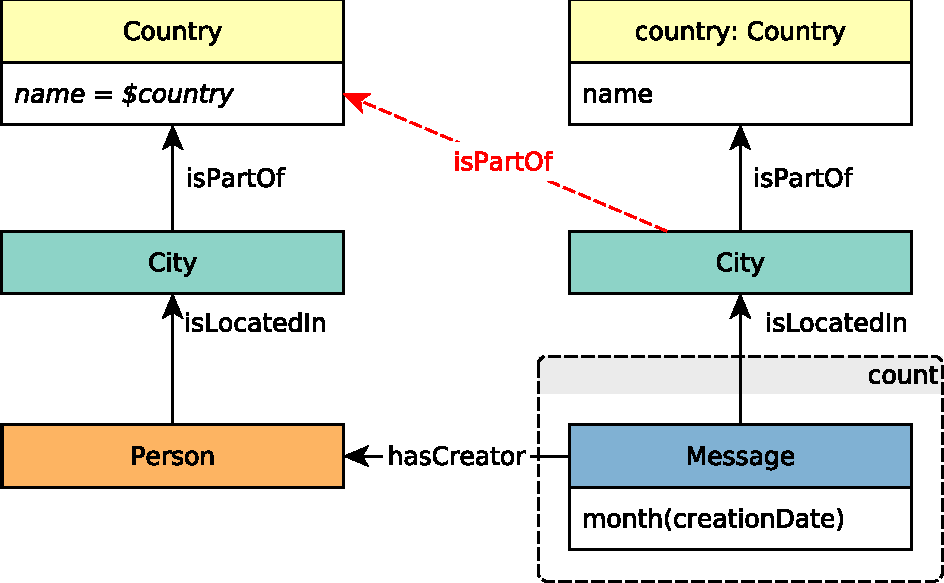
\includegraphics[scale=\patternscale,margin=0cm .2cm]{patterns/q23}
		\caption{Example graph pattern.}
		\label{fig:example-graph-pattern}
	\end{center}
\end{figure}



\section{Business Intelligence Queries}

\clearpage

\renewcommand*{\arraystretch}{1.5}
\begin{tabularx}{15cm}{|p{2.1cm}@{\hskip 1ex}|@{\hskip 1ex}X|}
	\hline
	number      & 1                                                          \\ \hline
	title       & Posting summary                                                           \\ \hline
	\multicolumn{2}{|c|}{ \includegraphics[scale=\patternscale,margin=0cm .2cm]{patterns/q01}} \\ \hline
	description & Given a date, find all Messages created before that date. Group them by
a 3-level grouping:

\begin{enumerate}
\def\labelenumi{\arabic{enumi}.}
\tightlist
\item
  by year of creation
\item
  for each year, group into message types, i.e., Posts or Comments
\item
  for each year-type group, split into four groups based on length of
  their content

  \begin{itemize}
  \tightlist
  \item
    0 \textless{}= length \textless{} 40: \texttt{short}
  \item
    40 \textless{}= length \textless{} 80: \texttt{one\ liner}
  \item
    80 \textless{}= length \textless{} 160: \texttt{tweet}
  \item
    160 \textless{}= length: \texttt{long}
  \end{itemize}
\end{enumerate}
 \\ \hline
	
	group       &
	\multicolumn{1}{>{\raggedright}X|}{
		\varname{year}, 
		\varname{message type}, 
		\varname{length group}
		}\\ \hline
	
	parameters  &
	\multicolumn{1}{>{\raggedright}X|}{
		\variable{date}{Date} 
		}\\ \hline
	result      &
	\multicolumn{1}{>{\raggedright}X|}{
		\variable{message.year}{32bitInteger}\\
		\variable{message type}{String}\\
		\variable{length category}{String}\\
		\variable{message count}{32bitInteger}\\
		\variable{average message length}{32bitInteger}\\
		\variable{sum message length}{32bitInteger}\\
		\variable{per messages}{32bitFloat}
		}\\ \hline
	sort        &
	\multicolumn{1}{>{\raggedright}X|}{
		\sortentry{year}{\desc}\\
		\sortentry{message type}{\asc}\\
		\sortentry{size category}{\asc}
		}\\ \hline
	choke points        &
	\multicolumn{1}{>{\raggedright}X|}{
		\chokepoint{1.2}, 
		\chokepoint{3.2}, 
		\chokepoint{4.1}
		}\\ \hline
\end{tabularx}
\clearpage

\renewcommand*{\arraystretch}{1.5}
\begin{tabularx}{15cm}{|p{2.1cm}@{\hskip 1ex}|@{\hskip 1ex}X|}
	\hline
	number      & 2                                                          \\ \hline
	title       & Top tags for country, age, gender, time                                                           \\ \hline
	\multicolumn{2}{|c|}{ 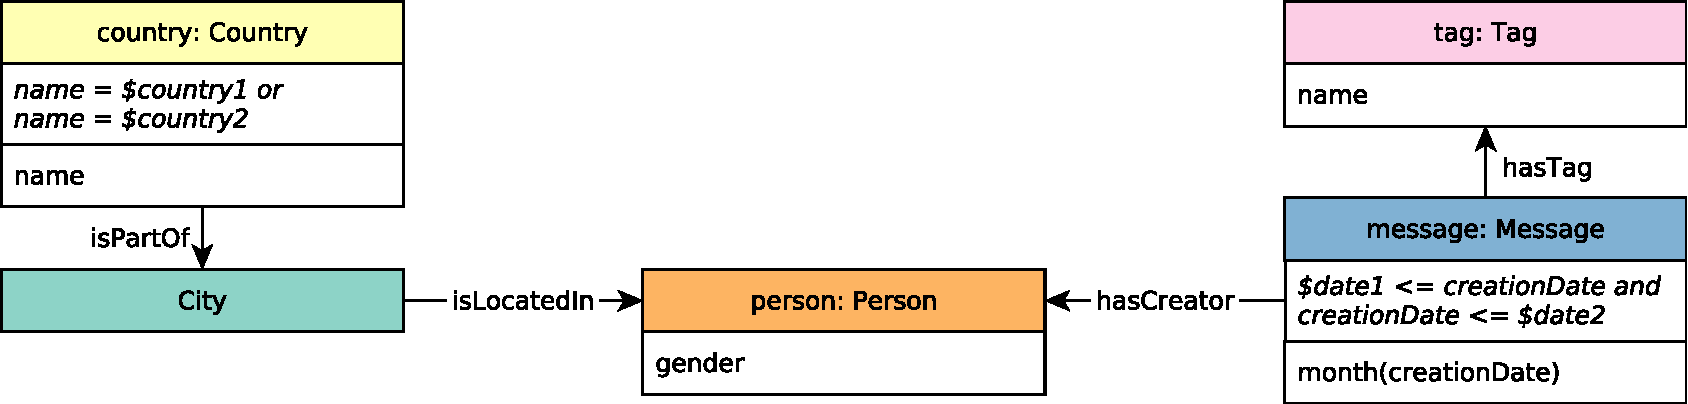
\includegraphics[scale=\patternscale,margin=0cm .2cm]{patterns/q02}} \\ \hline
	description & Select all Messages (Posts \& Comments) created between date1-date2
(inclusive) by persons located in country1 or country2. Select the
creators (Persons) and the Tags of these Messages. Split these Persons,
Tags and Messages into a 5-level grouping:

\begin{enumerate}
\def\labelenumi{\arabic{enumi}.}
\tightlist
\item
  name of country of person
\item
  month message was created
\item
  gender of person
\item
  age group of person, defined as years between person's birthday and
  end of simulation (2013-01-01), divided by 5, rounded down
\item
  name of tag attached to message
\end{enumerate}

Only return groups where number of messages is greater than 100.
 \\ \hline
	
	group       &
	\multicolumn{1}{>{\raggedright}X|}{
		\varname{countryName}, 
		\varname{month}, 
		\varname{gender}, 
		\varname{age group}, 
		\varname{name}
		}\\ \hline
	
	parameters  &
	\multicolumn{1}{>{\raggedright}X|}{
		\variable{date1}{Date} \\
		\variable{date2}{Date} \\
		\variable{country1}{String} \\
		\variable{country2}{String} 
		}\\ \hline
	result      &
	\multicolumn{1}{>{\raggedright}X|}{
		\variable{country.name}{String}\\
		\variable{message.month}{32bitInteger}\\
		\variable{person.gender}{String}\\
		\variable{ageGroup}{32bitInteger}\\
		\variable{tag.name}{String}\\
		\variable{messageCount}{64bitInteger}
		}\\ \hline
	sort        &
	\multicolumn{1}{>{\raggedright}X|}{
		\sortentry{messageCount}{\desc}\\
		\sortentry{tag.name}{\asc}\\
		\sortentry{ageGroup}{\asc}\\
		\sortentry{person.gender}{\asc}\\
		\sortentry{message.month}{\asc}\\
		\sortentry{country.name}{\asc}
		}\\ \hline
	limit       & 100                                                           \\ \hline
	choke points        &
	\multicolumn{1}{>{\raggedright}X|}{
		\chokepoint{1.1}, 
		\chokepoint{1.2}, 
		\chokepoint{1.4}, 
		\chokepoint{2.1}, 
		\chokepoint{2.3}, 
		\chokepoint{3.1}, 
		\chokepoint{3.2}
		}\\ \hline
\end{tabularx}
\clearpage

\input{query-cards/q03}
\renewcommand*{\arraystretch}{1.5}
\begin{tabularx}{15cm}{|p{2.1cm}@{\hskip 1ex}|@{\hskip 1ex}X|}
	\hline
	number      & 4                                                          \\ \hline
	title       & Popular topics in a country                                                           \\ \hline
	\multicolumn{2}{|c|}{ 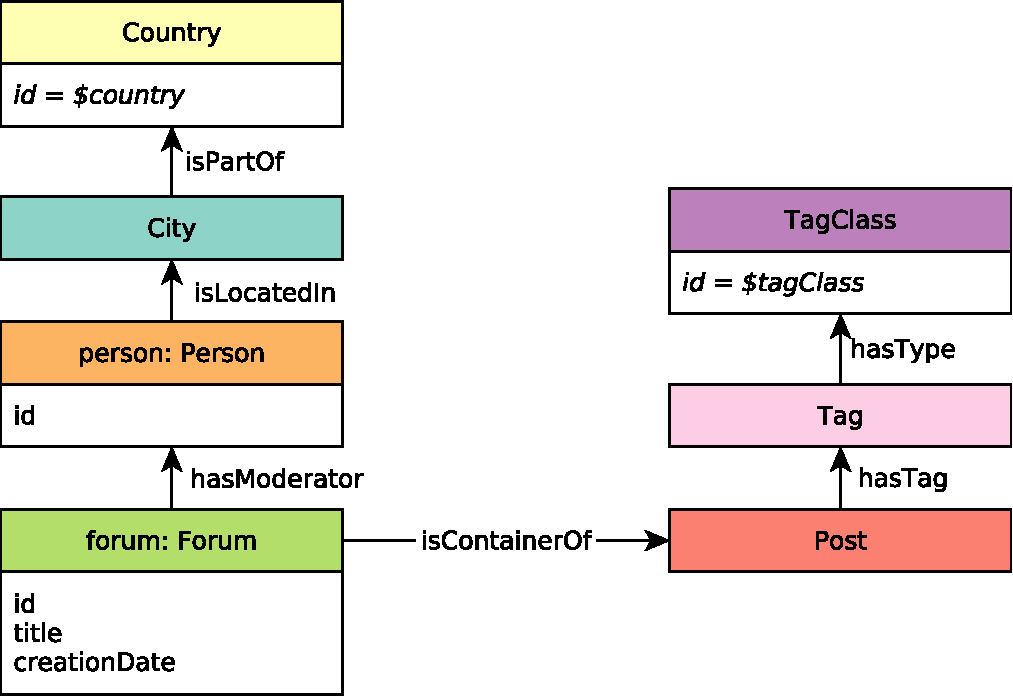
\includegraphics[scale=\patternscale,margin=0cm .2cm]{patterns/q04}} \\ \hline
	description & Given a TagClass and a Country, find all the Forums created in the given
Country, containing at least one Post with Tags belonging directly to
the given TagClass.

The location of a Forum is identified by the location of the Forum's
moderator.

TODO - what do we count, Posts? (szarnyasg)
 \\ \hline
	
	parameters  &
	\multicolumn{1}{>{\raggedright}X|}{
		\variable{tagClass}{32bitInteger} \\
		\variable{country}{32bitInteger} 
		}\\ \hline
	result      &
	\multicolumn{1}{>{\raggedright}X|}{
		\variable{forum.id}{64bitInteger}\\
		\variable{forum.title}{String}\\
		\variable{forum.creationDate}{DateTime}\\
		\variable{person.id}{64bitInteger}\\
		\variable{count}{32bitInteger}
		}\\ \hline
	sort        &
	\multicolumn{1}{>{\raggedright}X|}{
		\sortentry{count}{\desc}\\
		\sortentry{forum.id}{\asc}
		}\\ \hline
	limit       & 20                                                           \\ \hline
	choke points        &
	\multicolumn{1}{>{\raggedright}X|}{
		\chokepoint{1.1}, 
		\chokepoint{1.2}, 
		\chokepoint{1.4}, 
		\chokepoint{2.1}, 
		\chokepoint{2.2}, 
		\chokepoint{2.4}, 
		\chokepoint{3.3}
		}\\ \hline
\end{tabularx}
\clearpage

\renewcommand*{\arraystretch}{1.5}
\begin{tabularx}{15cm}{|p{2.1cm}@{\hskip 1ex}|@{\hskip 1ex}X|}
	\hline
	number      & 5                                                          \\ \hline
	title       & Top posters in a country                                                           \\ \hline
	\multicolumn{2}{|c|}{ 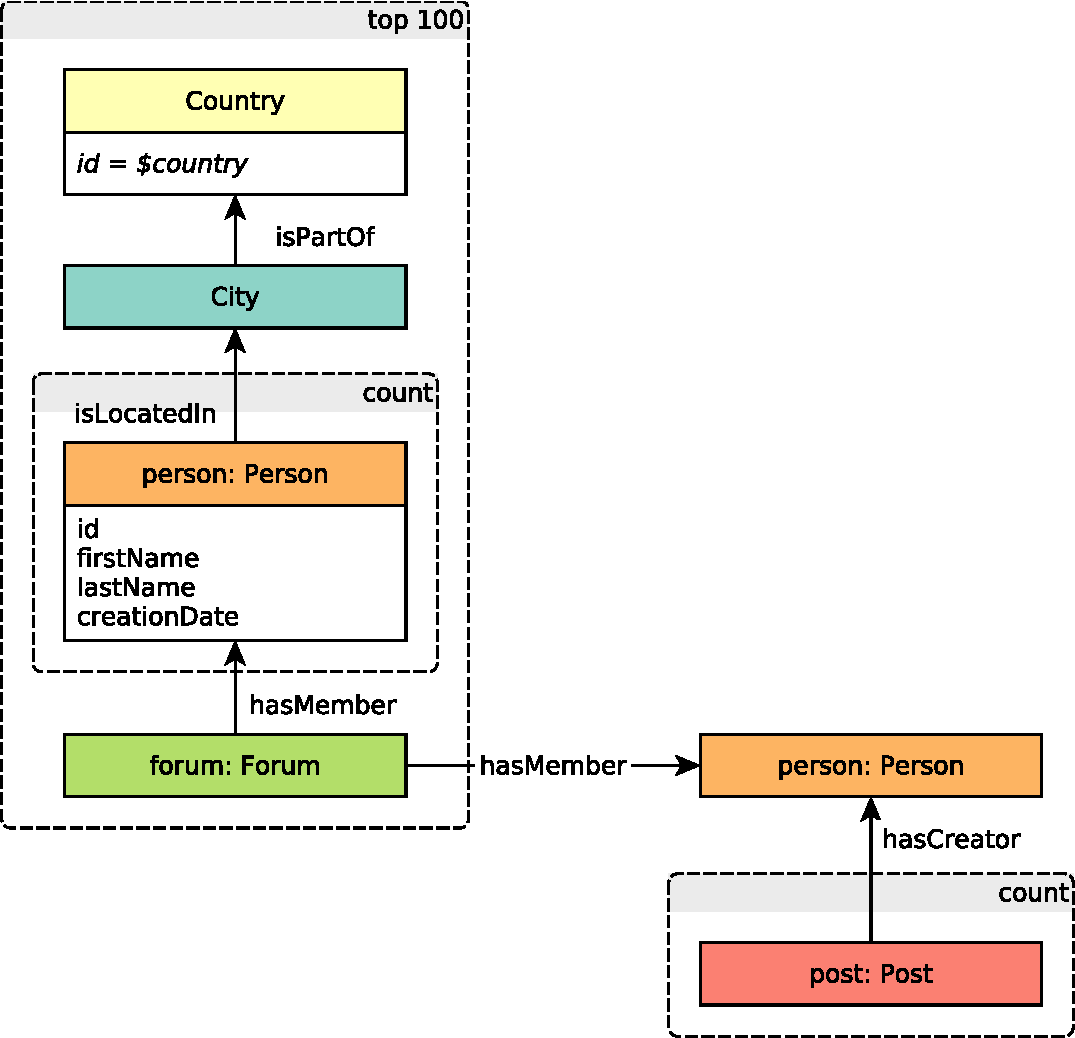
\includegraphics[scale=\patternscale,margin=0cm .2cm]{patterns/q05}} \\ \hline
	description & Find the most popular Forums for a given Country, where the popularity
of a Forum is measured by the number of members that Forum has from the
given Country.

For each member of the 100 most popular Forums, count the number of
Posts they made in any of those (most popular) Forums.
 \\ \hline
	
	group       &
	\multicolumn{1}{>{\raggedright}X|}{
		\varname{person.id}, 
		\varname{person.firstName}, 
		\varname{person.lastName}, 
		\varname{person.creationDate}
		}\\ \hline
	
	parameters  &
	\multicolumn{1}{>{\raggedright}X|}{
		\variable{country}{32bitInteger} 
		}\\ \hline
	result      &
	\multicolumn{1}{>{\raggedright}X|}{
		\variable{person.id}{64bitInteger}\\
		\variable{person.firstName}{String}\\
		\variable{person.lastName}{String}\\
		\variable{person.creationDate}{DateTime}\\
		\variable{postCount}{32bitInteger}
		}\\ \hline
	sort        &
	\multicolumn{1}{>{\raggedright}X|}{
		\sortentry{postCount}{\desc}\\
		\sortentry{person.id}{\asc}
		}\\ \hline
	limit       & 100                                                           \\ \hline
	choke points        &
	\multicolumn{1}{>{\raggedright}X|}{
		\chokepoint{1.2}, 
		\chokepoint{1.4}, 
		\chokepoint{1.5}, 
		\chokepoint{2.1}, 
		\chokepoint{2.2}, 
		\chokepoint{2.3}, 
		\chokepoint{2.4}, 
		\chokepoint{3.3}, 
		\chokepoint{5.3}, 
		\chokepoint{6.1}
		}\\ \hline
\end{tabularx}
\clearpage

\renewcommand*{\arraystretch}{1.5}
\begin{tabularx}{15cm}{|p{2.1cm}@{\hskip 1ex}|@{\hskip 1ex}X|}
	\hline
	number      & 6                                                          \\ \hline
	title       & Most active Posters of a given Topic                                                           \\ \hline
	\multicolumn{2}{|c|}{ 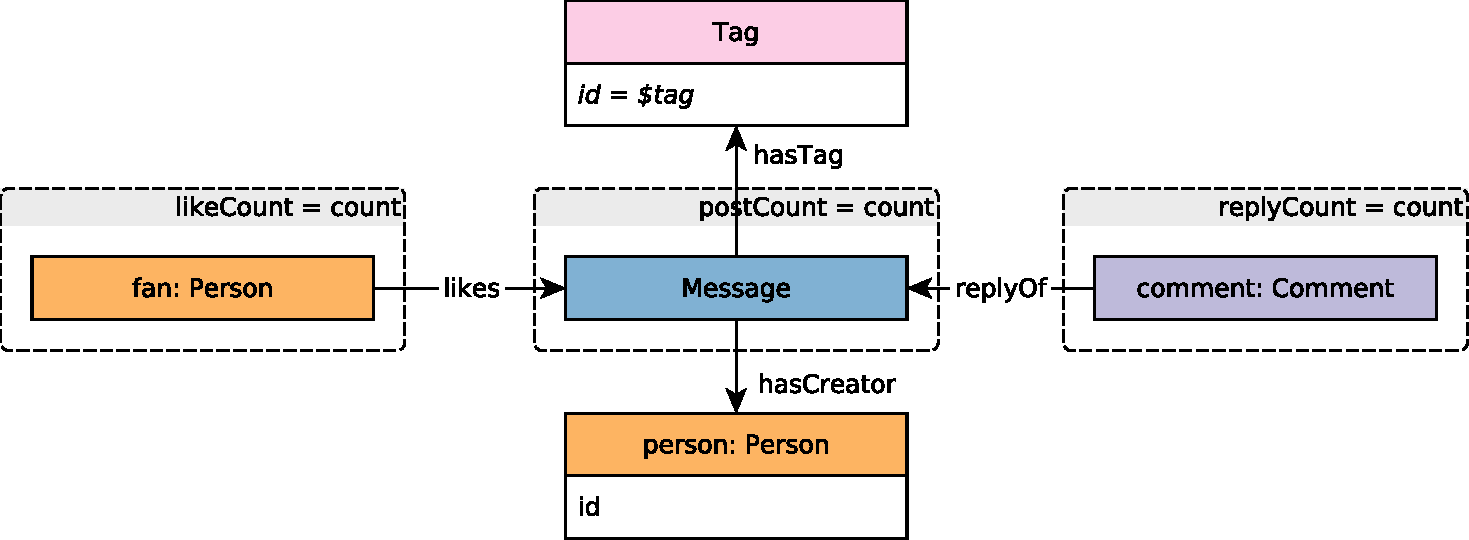
\includegraphics[scale=\patternscale,margin=0cm .2cm]{patterns/q06}} \\ \hline
	description & Get Persons who have created a Message (Post or Comment) with a given
Tag.

Each Person has a score, computed as follows:

\begin{itemize}
\tightlist
\item
  Count of Messages with the given Tag (\texttt{postCount}).
\item
  Count of Likes (\texttt{likeCount}) and Comments (\texttt{replyCount})
  in reply of their Messages with the given Tag. (TODO - transitive or
  direct? szarnyasg)
\end{itemize}

The sum is weighted as follows:

\begin{itemize}
\tightlist
\item
  Messages (\texttt{postCount}) are multiplied by 1,
\item
  Comments to Messages (\texttt{replyCount}) are multiplied by 2,
\item
  Likes (\texttt{likeCount}) are multiplied by 10.
\end{itemize}
 \\ \hline
	
	parameters  &
	\multicolumn{1}{>{\raggedright}X|}{
		\variable{tag}{32bitInteger} 
		}\\ \hline
	result      &
	\multicolumn{1}{>{\raggedright}X|}{
		\variable{person.id}{64bitInteger}\\
		\variable{replyCount}{32bitInteger}\\
		\variable{likeCount}{32bitInteger}\\
		\variable{postCount}{32bitInteger}\\
		\variable{score}{32bitInteger}
		}\\ \hline
	sort        &
	\multicolumn{1}{>{\raggedright}X|}{
		\sortentry{score}{\desc}\\
		\sortentry{person.id}{\asc}
		}\\ \hline
	limit       & 100                                                           \\ \hline
	choke points        &
	\multicolumn{1}{>{\raggedright}X|}{
		\chokepoint{1.2}, 
		\chokepoint{2.3}
		}\\ \hline
\end{tabularx}
\clearpage

\renewcommand*{\arraystretch}{1.5}
\begin{tabularx}{15cm}{|p{2.1cm}@{\hskip 1ex}|@{\hskip 1ex}X|}
	\hline
	number      & 7                                                          \\ \hline
	title       & Most authoritative users on a given topic                                                           \\ \hline
	\multicolumn{2}{|c|}{ 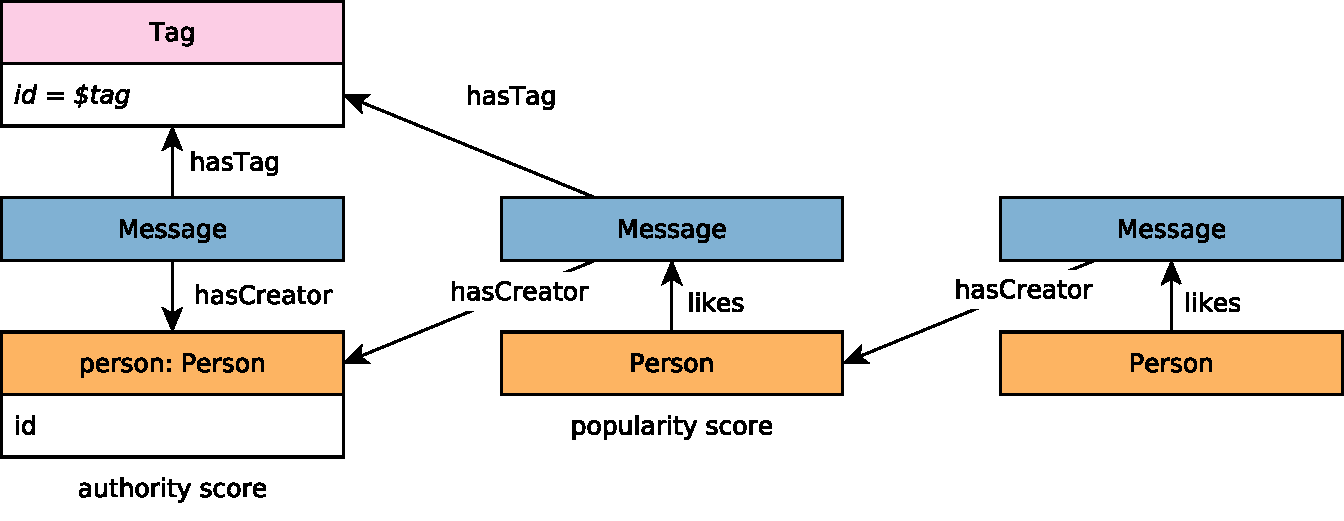
\includegraphics[scale=\patternscale,margin=0cm .2cm]{patterns/q07}} \\ \hline
	description & Given a Tag, find all Persons that ever created a Message with the given
Tag. For each of these Persons compute their ``authority score'' as
follows:

\begin{itemize}
\tightlist
\item
  The ``authority score'' is the sum of ``popularity scores'' of the
  Persons that liked any of that Person's Messages with the given Tag.
\item
  A Person's ``popularity score'' is defined as the total number of
  likes on all of their Messages.
\end{itemize}
 \\ \hline
	
	parameters  &
	\multicolumn{1}{>{\raggedright}X|}{
		\variable{tag}{32bitInteger} 
		}\\ \hline
	result      &
	\multicolumn{1}{>{\raggedright}X|}{
		\variable{person1.id}{64bitInteger}\\
		\variable{authorityScore}{32bitInteger}
		}\\ \hline
	sort        &
	\multicolumn{1}{>{\raggedright}X|}{
		\sortentry{authorityScore}{\desc}\\
		\sortentry{person1.id}{\asc}
		}\\ \hline
	limit       & 100                                                           \\ \hline
	choke points        &
	\multicolumn{1}{>{\raggedright}X|}{
		\chokepoint{1.2}, 
		\chokepoint{2.3}, 
		\chokepoint{3.2}, 
		\chokepoint{3.3}, 
		\chokepoint{6.1}
		}\\ \hline
\end{tabularx}
\clearpage

\renewcommand*{\arraystretch}{1.5}
\begin{tabularx}{15cm}{|p{2.1cm}@{\hskip 1ex}|@{\hskip 1ex}X|}
	\hline
	number      & 8                                                          \\ \hline
	title       & Related topics                                                           \\ \hline
	\multicolumn{2}{|c|}{ 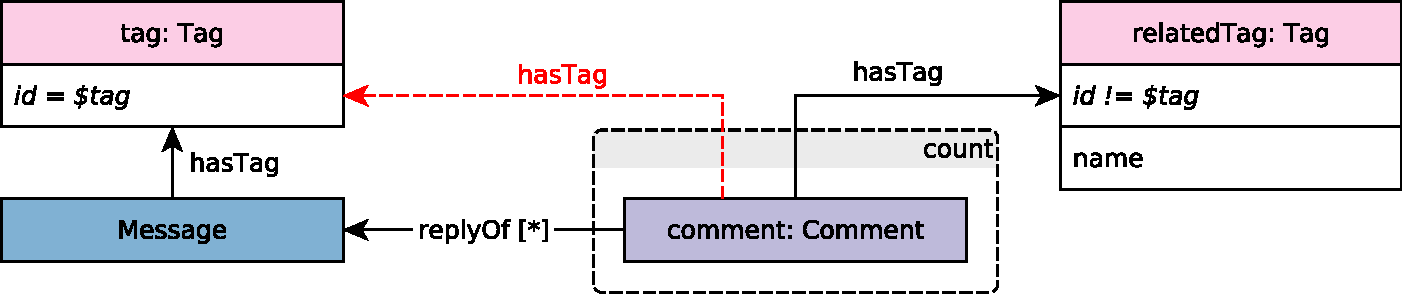
\includegraphics[scale=\patternscale,margin=0cm .2cm]{patterns/q08}} \\ \hline
	description & Find all Messages that have a given Tag. Find the related Tags attached
to replies of these Messages (TODO - transitive? szarnyasg), but only of
those replies that do not have the given Tag.

Group the Tags by name, and get the count of replies in each group.
 \\ \hline
	
	group       &
	\multicolumn{1}{>{\raggedright}X|}{
		\varname{relatedTag.name}
		}\\ \hline
	
	parameters  &
	\multicolumn{1}{>{\raggedright}X|}{
		\variable{tag}{32bitInteger} 
		}\\ \hline
	result      &
	\multicolumn{1}{>{\raggedright}X|}{
		\variable{relatedTag.name}{String}\\
		\variable{count}{32bitInteger}
		}\\ \hline
	sort        &
	\multicolumn{1}{>{\raggedright}X|}{
		\sortentry{count}{\desc}\\
		\sortentry{relatedTag.name}{\asc}
		}\\ \hline
	limit       & 100                                                           \\ \hline
	choke points        &
	\multicolumn{1}{>{\raggedright}X|}{
		\chokepoint{1.6}, 
		\chokepoint{3.3}, 
		\chokepoint{5.2}
		}\\ \hline
\end{tabularx}
\clearpage

\renewcommand*{\arraystretch}{1.5}
\begin{tabularx}{15cm}{|p{2.1cm}@{\hskip 1ex}|@{\hskip 1ex}X|}
	\hline
	number      & 9                                                          \\ \hline
	title       & Forum with related Tags                                                           \\ \hline
	\multicolumn{2}{|c|}{ 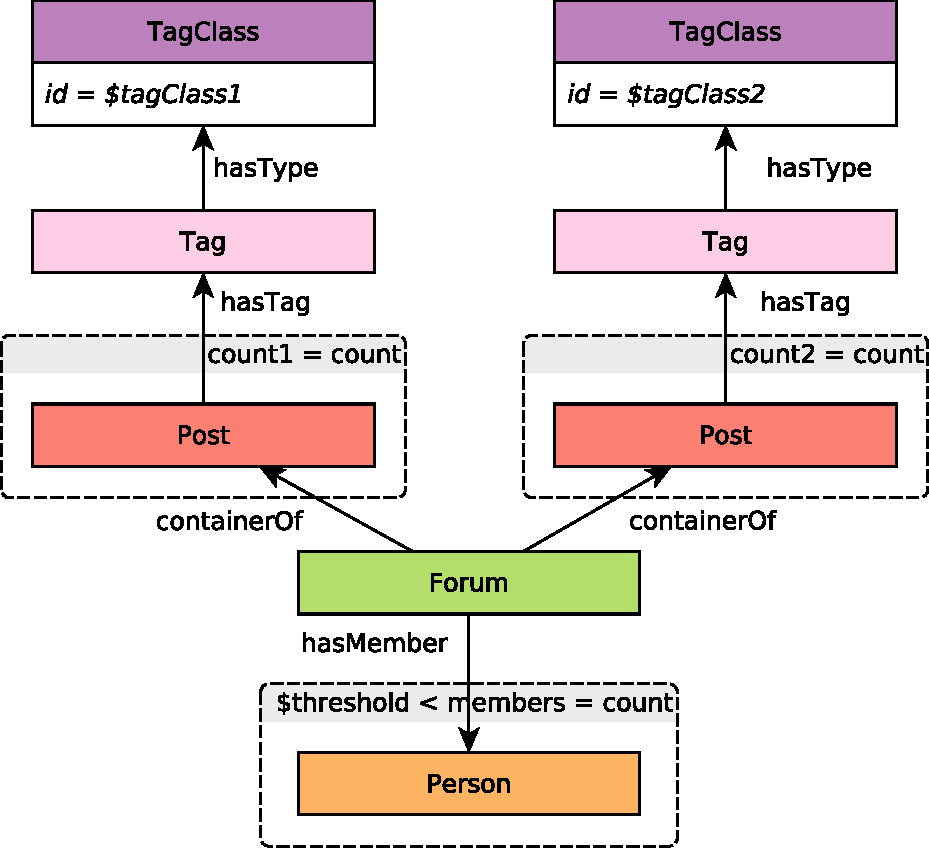
\includegraphics[scale=\patternscale,margin=0cm .2cm]{patterns/q09}} \\ \hline
	description & Given two TagClasses (\texttt{tagClass1} \& \texttt{tagClass2}), find
Forums that contain at least one Post with a Tag from \texttt{tagClass1}
and at least one Post with a Tag from \texttt{tagClass2} (direct
children not transitive) -- this may be the same Post.

Consider the Forums with a number of members greater than a given
threshold. For every such forum, count the number of Posts that have a
Tag from TagClass1 (count1), and the number of posts that have a tag
from TagClass2.
 \\ \hline
	
	parameters  &
	\multicolumn{1}{>{\raggedright}X|}{
		\variable{tagClass1}{32bitInteger} \\
		\variable{tagClass2}{32bitInteger} \\
		\variable{threshold}{32bitInteger} 
		}\\ \hline
	result      &
	\multicolumn{1}{>{\raggedright}X|}{
		\variable{forum.id}{64bitInteger}\\
		\variable{count1}{32bitInteger}Number of Posts with at least one tag belonging to tagClass1\\
		\variable{count2}{32bitInteger}Number of Posts with at least one tag belonging to tagClass2
		}\\ \hline
	sort        &
	\multicolumn{1}{>{\raggedright}X|}{
		\sortentry{count2}{\desc}\\
		\sortentry{count1}{\desc}\\
		\sortentry{forum.id}{\asc}
		}\\ \hline
	limit       & 100                                                           \\ \hline
	choke points        &
	\multicolumn{1}{>{\raggedright}X|}{
		\chokepoint{1.2}, 
		\chokepoint{1.4}, 
		\chokepoint{2.1}, 
		\chokepoint{2.3}, 
		\chokepoint{2.4}
		}\\ \hline
\end{tabularx}
\clearpage

\input{query-cards/q10}
\input{query-cards/q11}
\renewcommand*{\arraystretch}{1.5}
\begin{tabularx}{15cm}{|p{2.1cm}@{\hskip 1ex}|@{\hskip 1ex}X|}
	\hline
	number      & 12                                                          \\ \hline
	title       & Trending Posts                                                           \\ \hline
	\multicolumn{2}{|c|}{ \includegraphics[scale=\patternscale,margin=0cm .2cm]{patterns/q12}} \\ \hline
	description & Find all Messages created after a given date, that received more than a
given number of likes.
 \\ \hline
	
	parameters  &
	\multicolumn{1}{>{\raggedright}X|}{
		\variable{creationDate}{Date} \\
		\variable{likeThreshold}{32bitInteger} 
		}\\ \hline
	result      &
	\multicolumn{1}{>{\raggedright}X|}{
		\variable{message.id}{64bitInteger}\\
		\variable{message.creationDate}{DateTime}\\
		\variable{creator.firstName}{String}The first name of the post's creator\\
		\variable{creator.lastName}{String}The last name of the post's creator\\
		\variable{likeCount}{32bitInteger}The number of Likes the Post received
		}\\ \hline
	sort        &
	\multicolumn{1}{>{\raggedright}X|}{
		\sortentry{likeCount}{\desc}\\
		\sortentry{message.id}{\asc}
		}\\ \hline
	limit       & 100                                                           \\ \hline
	choke points        &
	\multicolumn{1}{>{\raggedright}X|}{
		\chokepoint{1.2}, 
		\chokepoint{2.2}, 
		\chokepoint{3.1}, 
		\chokepoint{6.1}
		}\\ \hline
\end{tabularx}
\clearpage

\renewcommand*{\arraystretch}{1.5}
\begin{tabularx}{15cm}{|p{2.1cm}@{\hskip 1ex}|@{\hskip 1ex}X|}
	\hline
	number      & 13                                                          \\ \hline
	title       & Popular Tags per month in a country                                                           \\ \hline
	\multicolumn{2}{|c|}{ \includegraphics[scale=\patternscale,margin=0cm .2cm]{patterns/q13}} \\ \hline
	description & Find all Messages in a given Country, as well as their Tags.

For each group, find the 5 most popular Tags, where popularity is the
number of Messages (from within the same group) where the Tag appears.
 \\ \hline
	
	group       &
	\multicolumn{1}{>{\raggedright}X|}{
		\varname{year}, 
		\varname{month}
		}\\ \hline
	
	parameters  &
	\multicolumn{1}{>{\raggedright}X|}{
		\variable{country}{String} 
		}\\ \hline
	result      &
	\multicolumn{1}{>{\raggedright}X|}{
		\variable{year}{32bitInteger}year(message.creationDate)\\
		\variable{month}{32bitInteger}month(message.creationDate)\\
		\variable{popularTags}{TagPairs}(tag.name - String, popularity - 32bitInteger), sorted descending by popularity, then ascending by tag name
		}\\ \hline
	sort        &
	\multicolumn{1}{>{\raggedright}X|}{
		\sortentry{year}{\desc}\\
		\sortentry{month}{\asc}
		}\\ \hline
	limit       & 100                                                           \\ \hline
	choke points        &
	\multicolumn{1}{>{\raggedright}X|}{
		\chokepoint{1.2}, 
		\chokepoint{2.2}, 
		\chokepoint{2.3}, 
		\chokepoint{3.2}, 
		\chokepoint{6.1}
		}\\ \hline
\end{tabularx}
\clearpage

\renewcommand*{\arraystretch}{1.5}
\begin{tabularx}{15cm}{|p{2.1cm}@{\hskip 1ex}|@{\hskip 1ex}X|}
	\hline
	number      & 14                                                          \\ \hline
	title       & Top thread initiators                                                           \\ \hline
	\multicolumn{2}{|c|}{ 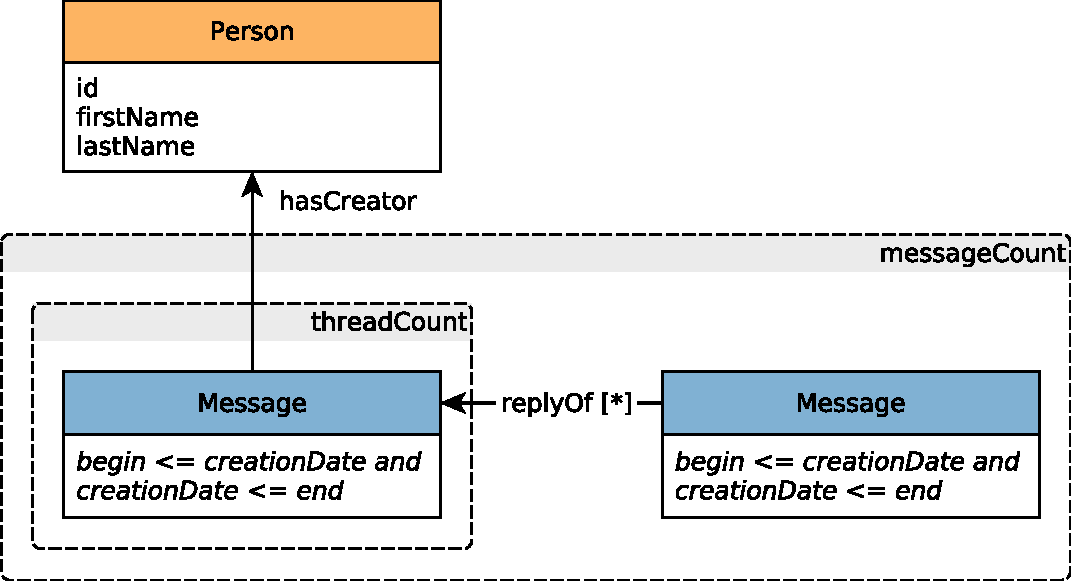
\includegraphics[scale=\patternscale,margin=0cm .2cm]{patterns/q14}} \\ \hline
	description & For each person, count the number Posts they created in the time
interval \texttt{(begin,\ end)}, and the number of messages in each of
their (transitive) reply trees. When calculating message counts only
consider messages created within the given time interval.

Return each person, number of Posts they created, and the count of all
messages that appeared in the reply trees (including Post at tree root)
they created.
 \\ \hline
	
	parameters  &
	\multicolumn{1}{>{\raggedright}X|}{
		\variable{begin}{Date} \\
		\variable{end}{Date} 
		}\\ \hline
	result      &
	\multicolumn{1}{>{\raggedright}X|}{
		\variable{person.id}{64bitInteger}\\
		\variable{person.firstName}{String}\\
		\variable{person.lastName}{String}\\
		\variable{threadCount}{32bitInteger}The number of threads initiated by that Person\\
		\variable{messageCount}{32bitInteger}The number of messages created in all the threads this Person initiated
		}\\ \hline
	sort        &
	\multicolumn{1}{>{\raggedright}X|}{
		\sortentry{messageCount}{\desc}\\
		\sortentry{person.id}{\asc}
		}\\ \hline
	limit       & 100                                                           \\ \hline
	choke points        &
	\multicolumn{1}{>{\raggedright}X|}{
		\chokepoint{1.2}, 
		\chokepoint{2.2}, 
		\chokepoint{2.3}, 
		\chokepoint{3.2}, 
		\chokepoint{7.2}, 
		\chokepoint{7.3}, 
		\chokepoint{7.4}
		}\\ \hline
\end{tabularx}
\clearpage

\input{query-cards/q15}
\renewcommand*{\arraystretch}{1.5}
\begin{tabularx}{15cm}{|p{2.1cm}@{\hskip 1ex}|@{\hskip 1ex}X|}
	\hline
	number      & 16                                                          \\ \hline
	title       & Experts in social circle                                                           \\ \hline
	\multicolumn{2}{|c|}{ 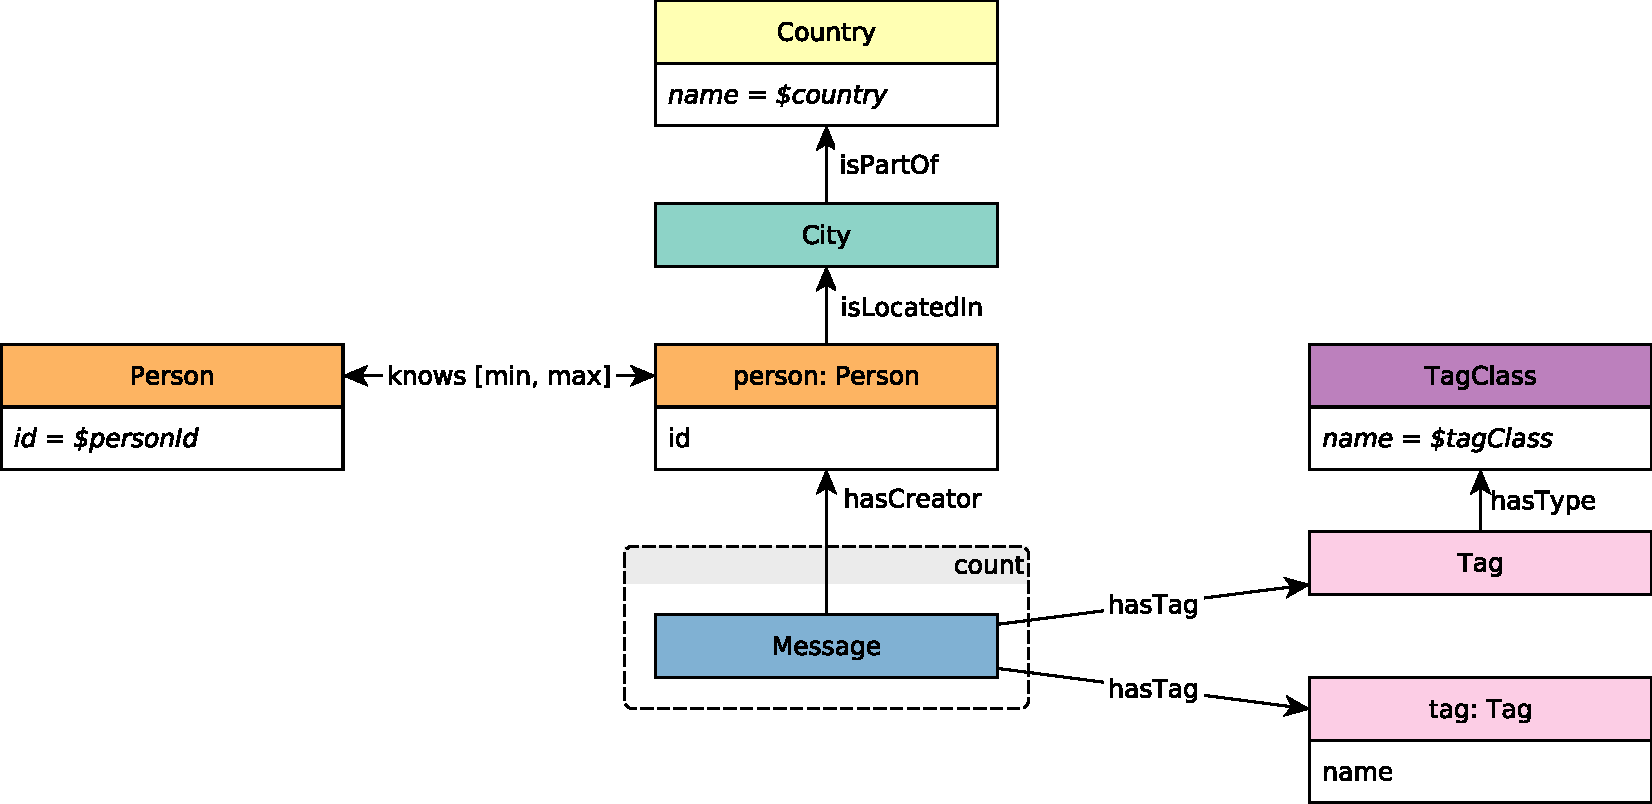
\includegraphics[scale=\patternscale,margin=0cm .2cm]{patterns/q16}} \\ \hline
	description & Given a Person, find all other Persons that live in a given country and
are connected to given person by a transitive path with length in range
\texttt{{[}min,\ max{]}} through the knows relation.

{[}DISCUSS: edge isomorphism semantics{]}

For each of these Persons, retrieve all of their Messages (Posts \&
Comments) that contain at least one Tag belonging to a given TagClass
(direct relation not transitive).

For each Message, also retrieve its Tags.

TODO {[}szarnyasg{]}: what is postCount?
 \\ \hline
	
	group       &
	\multicolumn{1}{>{\raggedright}X|}{
		\varname{tag.name}, 
		\varname{person.id}
		}\\ \hline
	
	parameters  &
	\multicolumn{1}{>{\raggedright}X|}{
		\variable{personId}{64bitInteger} \\
		\variable{country}{String} \\
		\variable{tagClass}{String} \\
		\variable{minPathDistance}{32bitInteger} \\
		\variable{maxPathDistance}{32bitInteger} 
		}\\ \hline
	result      &
	\multicolumn{1}{>{\raggedright}X|}{
		\variable{person.id}{64bitInteger}\\
		\variable{tag.name}{String}\\
		\variable{messageCount}{32bitInteger}number of Messages created by that Person containing that Tag
		}\\ \hline
	sort        &
	\multicolumn{1}{>{\raggedright}X|}{
		\sortentry{messageCount}{\desc}\\
		\sortentry{tag.name}{\asc}\\
		\sortentry{person.id}{\asc}
		}\\ \hline
	limit       & 100                                                           \\ \hline
	choke points        &
	\multicolumn{1}{>{\raggedright}X|}{
		\chokepoint{1.2}, 
		\chokepoint{1.4}, 
		\chokepoint{2.3}, 
		\chokepoint{2.4}, 
		\chokepoint{3.3}, 
		\chokepoint{7.2}, 
		\chokepoint{7.3}
		}\\ \hline
\end{tabularx}
\clearpage

\renewcommand*{\arraystretch}{1.5}
\begin{tabularx}{15cm}{|p{2.1cm}@{\hskip 1ex}|@{\hskip 1ex}X|}
	\hline
	number      & 17                                                          \\ \hline
	title       & Friend triangles                                                           \\ \hline
	\multicolumn{2}{|c|}{ 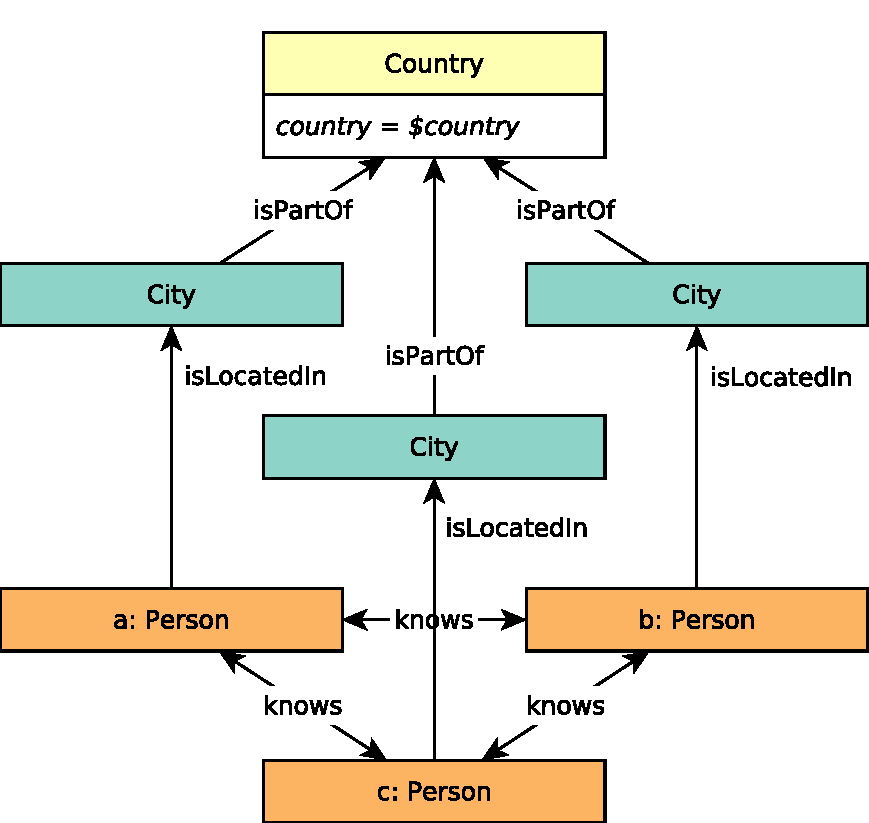
\includegraphics[scale=\patternscale,margin=0cm .2cm]{patterns/q17}} \\ \hline
	description & For a given country, count all the distinct triples of persons such that
\texttt{a} is friend of \texttt{b}, \texttt{b} is friend of \texttt{c},
and \texttt{c} is friend of \texttt{a}.

Distinct means that given a triple \emph{t1} in the result set \emph{R}
of all qualified triples, there is not a triple \emph{t2} in \emph{R}
such that \textbar{}\emph{t1} U \emph{b}\textbar{} = 3.
 \\ \hline
	
	parameters  &
	\multicolumn{1}{>{\raggedright}X|}{
		\variable{country}{String} 
		}\\ \hline
	result      &
	\multicolumn{1}{>{\raggedright}X|}{
		\variable{count}{32bitInteger}
		}\\ \hline
	choke points        &
	\multicolumn{1}{>{\raggedright}X|}{
		\chokepoint{1.1}, 
		\chokepoint{2.3}
		}\\ \hline
\end{tabularx}
\clearpage

\input{query-cards/q18}
\input{query-cards/q19}
\renewcommand*{\arraystretch}{1.5}
\begin{tabularx}{15cm}{|p{2.1cm}@{\hskip 1ex}|@{\hskip 1ex}X|}
	\hline
	number      & 20                                                          \\ \hline
	title       & High-level topics                                                           \\ \hline
	\multicolumn{2}{|c|}{ 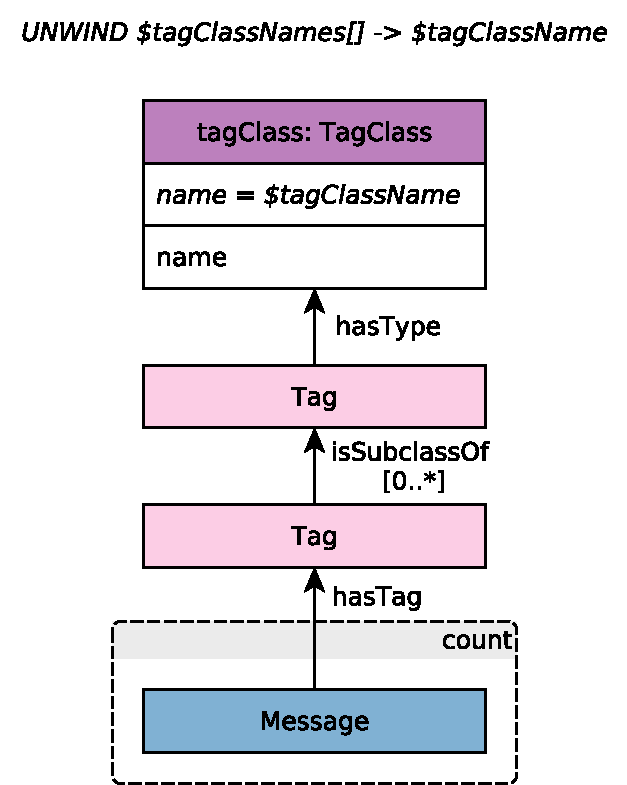
\includegraphics[scale=\patternscale,margin=0cm .2cm]{patterns/q20}} \\ \hline
	description & For all given TagClasses, count number of Messages that have a Tag that
belongs to that TagClass or any of its children (all descendants through
a transitive relation).
 \\ \hline
	
	parameters  &
	\multicolumn{1}{>{\raggedright}X|}{
		\variable{tagClasses}{String[]} 
		}\\ \hline
	result      &
	\multicolumn{1}{>{\raggedright}X|}{
		\variable{tagClass.name}{String}the TagClass of the root\\
		\variable{postCount}{32bitInteger}
		}\\ \hline
	sort        &
	\multicolumn{1}{>{\raggedright}X|}{
		\sortentry{postCount}{\desc}\\
		\sortentry{tagClass.name}{\asc}
		}\\ \hline
	limit       & 100                                                           \\ \hline
	choke points        &
	\multicolumn{1}{>{\raggedright}X|}{
		\chokepoint{1.6}, 
		\chokepoint{2.1}, 
		\chokepoint{6.1}
		}\\ \hline
\end{tabularx}
\clearpage

\renewcommand*{\arraystretch}{1.5}
\begin{tabularx}{15cm}{|p{2.1cm}@{\hskip 1ex}|@{\hskip 1ex}X|}
	\hline
	number      & 21                                                          \\ \hline
	title       & Zombies in a country                                                           \\ \hline
	\multicolumn{2}{|c|}{ \includegraphics[scale=\patternscale,margin=0cm .2cm]{patterns/q21}} \\ \hline
	description & Find zombies within the given country, and return their zombie scores.

A zombie is a Person created before the given \texttt{endDate} and that
has created between \texttt{{[}0,\ 1)} Messages per month, on average,
during the time range between profile creation date and the given
\texttt{endDate}.

The number of months spans the time range from creation date of the
profile to the \texttt{endDate} and also includes partial months.
 \\ \hline
	
	parameters  &
	\multicolumn{1}{>{\raggedright}X|}{
		\variable{country}{String} \\
		\variable{endDate}{Date} 
		}\\ \hline
	result      &
	\multicolumn{1}{>{\raggedright}X|}{
		\variable{person.id}{64bitInteger}\\
		\variable{zombieLikeCount}{32bitInteger}\\
		\variable{realLikeCount}{32bitInteger}\\
		\variable{zombieScore}{32bitFloat}the ratio between the number of likes received from zombies (`zombieLikeCount`) and the total number of likes received on that person's messages (`realLikeCount`) -- only count likes received from profiles that were created before the given `endDate`.
		}\\ \hline
	sort        &
	\multicolumn{1}{>{\raggedright}X|}{
		\sortentry{zombieScore}{\desc}\\
		\sortentry{person.id}{\asc}
		}\\ \hline
	limit       & 100                                                           \\ \hline
	choke points        &
	\multicolumn{1}{>{\raggedright}X|}{
		\chokepoint{1.2}, 
		\chokepoint{2.1}, 
		\chokepoint{2.3}, 
		\chokepoint{2.4}, 
		\chokepoint{3.2}, 
		\chokepoint{3.3}, 
		\chokepoint{5.1}, 
		\chokepoint{5.3}
		}\\ \hline
\end{tabularx}
\clearpage

\renewcommand*{\arraystretch}{1.5}
\begin{tabularx}{15cm}{|p{2.1cm}@{\hskip 1ex}|@{\hskip 1ex}X|}
	\hline
	number      & 22                                                          \\ \hline
	title       & International dialog                                                           \\ \hline
	\multicolumn{2}{|c|}{ 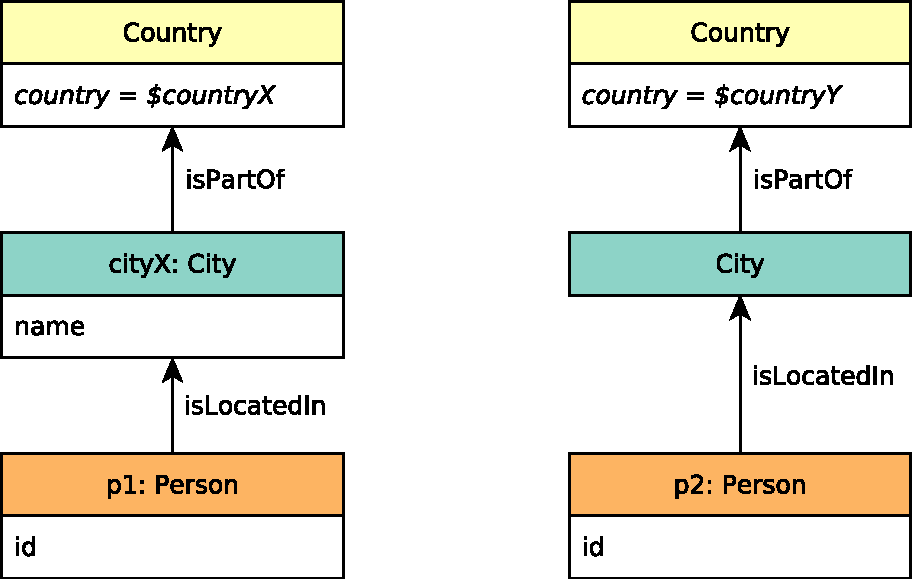
\includegraphics[scale=\patternscale,margin=0cm .2cm]{patterns/q22}} \\ \hline
	description & Consider all pairs of people \texttt{(p1,\ p2)} such that one is located
in a city of Country \texttt{countryX} and the other is located in a
city of Country \texttt{countryY}.

For each city of Country \texttt{countryX}, return the highest scoring
pair.

The score of a pair is defined as the sum of the scores of the following
kinds of interaction:

\begin{itemize}
\tightlist
\item
  \texttt{p1} has created a reply Comment to at least one Comment or
  Post by \texttt{p2}: \texttt{Score\ =\ 4}
\item
  \texttt{p1} has created at least one Post or Comment that \texttt{p2}
  has created a reply Comment to: \texttt{Score\ =\ 1}
\item
  \texttt{p1} and \texttt{p2} Know each other: \texttt{Score\ =\ 15}
\item
  \texttt{p1} liked at least one Post or Comment by \texttt{p2}:
  \texttt{Score\ =\ 10}
\item
  \texttt{p1} has created at least one Post or Comment that was liked by
  \texttt{p2}: \texttt{Score\ =\ 1}
\end{itemize}

I.e., the maximum score a pair can obtain is:
\texttt{4\ +\ 1\ +\ 15\ +\ 10\ +\ 1\ =\ 31}
 \\ \hline
	
	parameters  &
	\multicolumn{1}{>{\raggedright}X|}{
		\variable{countryX}{String} \\
		\variable{countryY}{String} 
		}\\ \hline
	result      &
	\multicolumn{1}{>{\raggedright}X|}{
		\variable{p1.id}{64bitInteger}\\
		\variable{p2.id}{64bitInteger}\\
		\variable{cityX.name}{String}\\
		\variable{score}{32bitInteger}
		}\\ \hline
	sort        &
	\multicolumn{1}{>{\raggedright}X|}{
		\sortentry{score}{\desc}\\
		\sortentry{p1.id}{\asc}\\
		\sortentry{p2.id}{\asc}
		}\\ \hline
	choke points        &
	\multicolumn{1}{>{\raggedright}X|}{
		\chokepoint{1.4}, 
		\chokepoint{1.6}, 
		\chokepoint{2.1}, 
		\chokepoint{3.1}, 
		\chokepoint{3.3}, 
		\chokepoint{5.1}, 
		\chokepoint{5.2}, 
		\chokepoint{5.3}
		}\\ \hline
\end{tabularx}
\clearpage

\renewcommand*{\arraystretch}{1.5}
\begin{tabularx}{15cm}{|p{2.1cm}@{\hskip 1ex}|@{\hskip 1ex}X|}
	\hline
	number      & 23                                                          \\ \hline
	title       & Holiday destinations                                                           \\ \hline
	\multicolumn{2}{|c|}{ 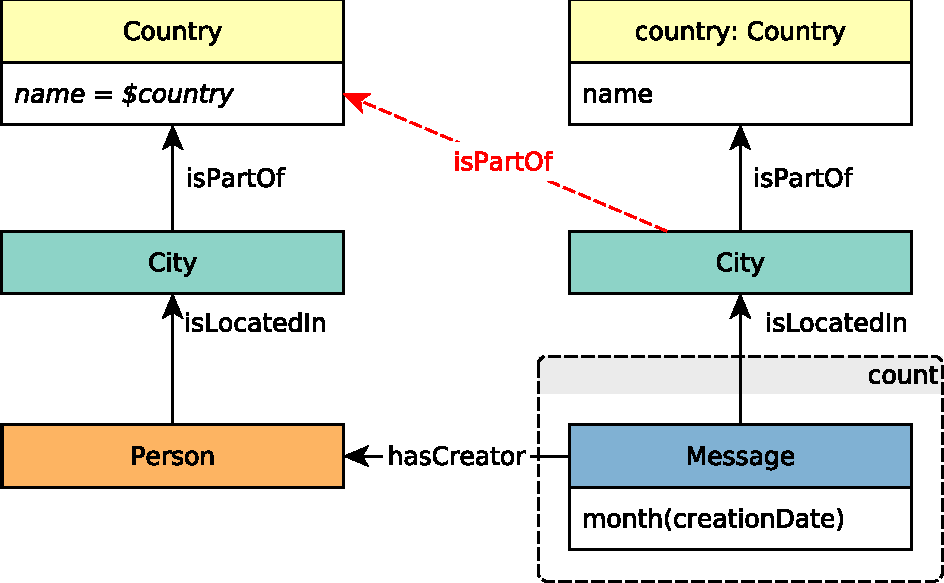
\includegraphics[scale=\patternscale,margin=0cm .2cm]{patterns/q23}} \\ \hline
	description & Count the messages all residents of Country \texttt{country} have
written abroad grouped by month and Country. A Message was written
abroad if the Country the Message was written in is different than the
Country of the Person it was written by.
 \\ \hline
	
	parameters  &
	\multicolumn{1}{>{\raggedright}X|}{
		\variable{country}{String} 
		}\\ \hline
	result      &
	\multicolumn{1}{>{\raggedright}X|}{
		\variable{messageCount}{32bitInteger}The number of messages in each group\\
		\variable{country.name}{String}The name of the destination country\\
		\variable{month}{32bitInteger}
		}\\ \hline
	sort        &
	\multicolumn{1}{>{\raggedright}X|}{
		\sortentry{messageCount}{\desc}\\
		\sortentry{country.name}{\asc}\\
		\sortentry{month}{\asc}
		}\\ \hline
	limit       & 100                                                           \\ \hline
	choke points        &
	\multicolumn{1}{>{\raggedright}X|}{
		\chokepoint{1.6}, 
		\chokepoint{2.3}, 
		\chokepoint{2.4}, 
		\chokepoint{3.3}, 
		\chokepoint{4.3}
		}\\ \hline
\end{tabularx}
\clearpage

\renewcommand*{\arraystretch}{1.5}
\begin{tabularx}{15cm}{|p{2.1cm}@{\hskip 1ex}|@{\hskip 1ex}X|}
	\hline
	number      & 24                                                          \\ \hline
	title       & Messages by Topic and Continent                                                           \\ \hline
	\multicolumn{2}{|c|}{ 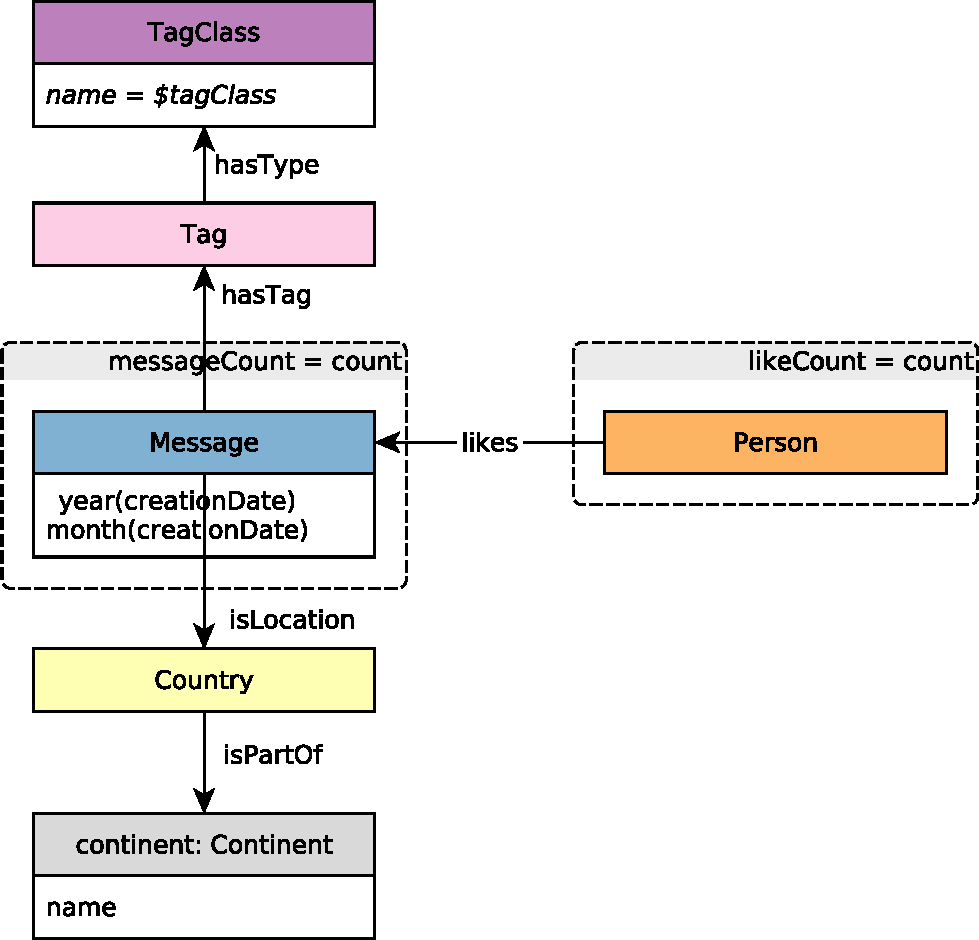
\includegraphics[scale=\patternscale,margin=0cm .2cm]{patterns/q24}} \\ \hline
	description & Find all Messages tagged with a Tag from the given TagClass
(non-transitive).

Count all messages and their likes grouped by continent, year, and
month. (TODO - do we group the Messages or the Persons who liked the
Messages by continent? I think the former one - szarnyasg)
 \\ \hline
	
	group       &
	\multicolumn{1}{>{\raggedright}X|}{
		\varname{year}, 
		\varname{month}, 
		\varname{continent.name}
		}\\ \hline
	
	parameters  &
	\multicolumn{1}{>{\raggedright}X|}{
		\variable{tagClass}{String} 
		}\\ \hline
	result      &
	\multicolumn{1}{>{\raggedright}X|}{
		\variable{messageCount}{32bitInteger}\\
		\variable{likeCount}{32bitInteger}\\
		\variable{year}{32bitInteger}year of the Message's creationDate\\
		\variable{month}{32bitInteger}month of the Message's creationDate\\
		\variable{continent.name}{String}
		}\\ \hline
	sort        &
	\multicolumn{1}{>{\raggedright}X|}{
		\sortentry{year}{\asc}\\
		\sortentry{month}{\asc}\\
		\sortentry{continent.name}{\desc}
		}\\ \hline
	limit       & 100                                                           \\ \hline
	choke points        &
	\multicolumn{1}{>{\raggedright}X|}{
		\chokepoint{1.6}, 
		\chokepoint{2.1}, 
		\chokepoint{2.3}, 
		\chokepoint{2.4}, 
		\chokepoint{3.2}, 
		\chokepoint{4.3}
		}\\ \hline
\end{tabularx}
\clearpage

\renewcommand*{\arraystretch}{1.5}
\begin{tabularx}{15cm}{|p{2.1cm}@{\hskip 1ex}|@{\hskip 1ex}X|}
	\hline
	number      & 25                                                          \\ \hline
	title       & Weighted paths                                                           \\ \hline
	\multicolumn{2}{|c|}{ 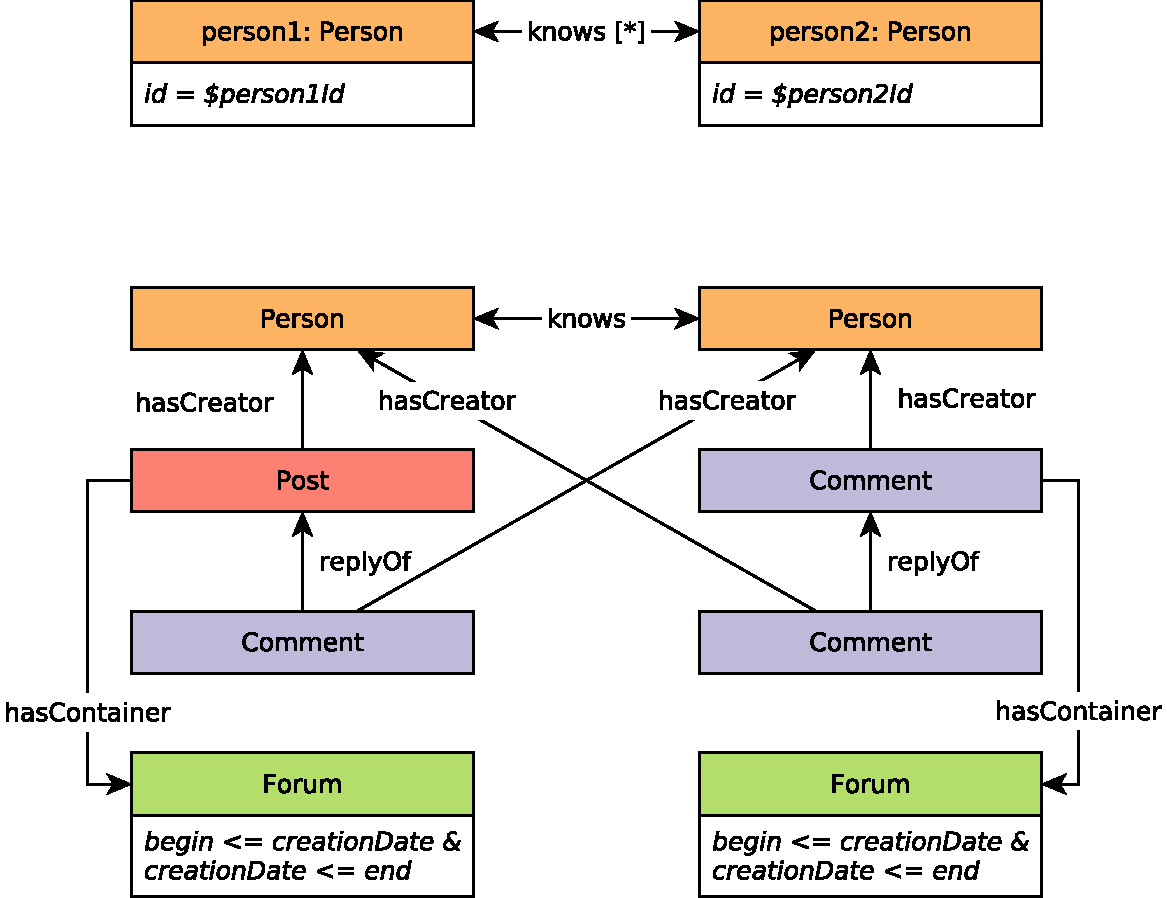
\includegraphics[scale=\patternscale,margin=0cm .2cm]{patterns/q25}} \\ \hline
	description & Given two Persons, find all (unweighted) shortest paths between these
two Persons, in the subgraph induced by the Knows relationship.

Then, for each path calculate a weight. The nodes in the path are
Persons, and the weight of a path is the sum of weights between every
pair of consecutive Person nodes in the path.

The weight for a pair of Persons is calculated such that every reply (by
one of the Persons) to a Post (by the other Person) contributes 1.0, and
every reply (by ones of the Persons) to a Comment (by the other Person)
contributes 0.5.

Only consider messages that were created in a forum that was created
within the timeframe \texttt{{[}startDate,\ endDate{]}}.

Return all the paths with shortest length, and their weights.
 \\ \hline
	
	parameters  &
	\multicolumn{1}{>{\raggedright}X|}{
		\variable{person1Id}{64bitInteger} \\
		\variable{person2Id}{64bitInteger} \\
		\variable{startDate}{Date} \\
		\variable{endDate}{Date} 
		}\\ \hline
	result      &
	\multicolumn{1}{>{\raggedright}X|}{
		\variable{person.id}{64bitInteger}Identifiers representing an ordered sequence of the Persons in the path weight
		}\\ \hline
	sort        &
	\multicolumn{1}{>{\raggedright}X|}{
		\sortentry{weight}{\desc}The order of paths with the same weight is unspecified
		}\\ \hline
	choke points        &
	\multicolumn{1}{>{\raggedright}X|}{
		\chokepoint{1.2}, 
		\chokepoint{2.1}, 
		\chokepoint{2.2}, 
		\chokepoint{2.4}, 
		\chokepoint{3.3}, 
		\chokepoint{5.1}, 
		\chokepoint{5.3}, 
		\chokepoint{7.2}, 
		\chokepoint{7.3}
		}\\ \hline
\end{tabularx}
\clearpage

